%%%%%%%%%%%%%%%%%%%%%%%%%%%%%%%%%%%%%%%%%
% Beamer Presentation
% LaTeX Template
% Version 1.0 (10/11/12)
%
% This template has been downloaded from:
% http://www.LaTeXTemplates.com
%
% License:
% CC BY-NC-SA 3.0 (http://creativecommons.org/licenses/by-nc-sa/3.0/)
%
%%%%%%%%%%%%%%%%%%%%%%%%%%%%%%%%%%%%%%%%%

%----------------------------------------------------------------------------------------
%	PACKAGES AND THEMES
%----------------------------------------------------------------------------------------

\documentclass{beamer}

\mode<presentation> {

% The Beamer class comes with a number of default slide themes
% which change the colors and layouts of slides. Below this is a list
% of all the themes, uncomment each in turn to see what they look like.

%\usetheme{default}
%\usetheme{AnnArbor}
%\usetheme{Antibes}
%\usetheme{Bergen}
%\usetheme{Berkeley}
%\usetheme{Berlin}
%\usetheme{Boadilla}
%\usetheme{CambridgeUS}
%\usetheme{Copenhagen}
%\usetheme{Darmstadt}
%\usetheme{Dresden}
%\usetheme{Frankfurt}
%\usetheme{Goettingen}
%\usetheme{Hannover}
%\usetheme{Ilmenau}
%\usetheme{JuanLesPins}
%\usetheme{Luebeck}
%\usetheme{Madrid}
%\usetheme{Malmoe}
%\usetheme{Marburg}
%\usetheme{Montpellier}
%\usetheme{PaloAlto}
%\usetheme{Pittsburgh}
%\usetheme{Rochester}
%\usetheme{Singapore}
\usetheme{Szeged}
%\usetheme{Warsaw}

% As well as themes, the Beamer class has a number of color themes
% for any slide theme. Uncomment each of these in turn to see how it
% changes the colors of your current slide theme.

%\usecolortheme{albatross}
%\usecolortheme{beaver}
%\usecolortheme{beetle}
%\usecolortheme{crane}
%\usecolortheme{dolphin}
%\usecolortheme{dove}
%\usecolortheme{fly}
%\usecolortheme{lily}
%\usecolortheme{orchid}
%\usecolortheme{rose}
%\usecolortheme{seagull}
%\usecolortheme{seahorse}
%\usecolortheme{whale}
%\usecolortheme{wolverine}
%\usecolortheme{spruce}

%\setbeamertemplate{footline} % To remove the footer line in all slides uncomment this line
%\setbeamertemplate{footline}[page number] % To replace the footer line in all slides with a simple slide count uncomment this line

%\setbeamertemplate{navigation symbols}{} % To remove the navigation symbols from the bottom of all slides uncomment this line
}

\usepackage{graphicx} % Allows including images
\usepackage{booktabs} % Allows the use of \toprule, \midrule and \bottomrule in tables
\usepackage{verbatim}

%----------------------------------------------------------------------------------------
%	TITLE PAGE
%----------------------------------------------------------------------------------------

\title[MASON and ECJ]{Doing Some Interesting Experiments with\\ ECJ and MASON Toolkit} % The short title appears at the bottom of every slide, the full title is only on the title page

% This logo will appear on every page.
\logo{%
    
\includegraphics[width=2cm,keepaspectratio]{logomsug-cmyk.pdf}~%
    
\includegraphics[width=1.5cm,keepaspectratio]{coin-logo.pdf}%    
}

\author{Presenter: Khaled} % Your name
\institute[COIN Laboratory, MSU] % Your institution as it will appear on the bottom of every slide, may be shorthand to save space
{
Computational Optimization and Innovation (COIN) Laboratory \\
Michigan State University \\ % Your institution for the title page
\medskip
\textit{talukde1@msu.edu} \\ % Your email address
%\medskip
%\emph{Some portion of this slide is taken from Prof. Sean's talk}
}

%\date{\today} % Date, can be changed to a custom date
% \date{June 16, 2013}
\date{April 28, 2017}

\graphicspath{%
	% {../figs/}%
	% {../data/}%
	{./figs/}%
	% {../../../report/figs/}%
	% {./}%
}

\begin{document}

\begin{frame}
\titlepage % Print the title page as the first slide
\end{frame}

%\begin{frame}
%\frametitle{Overview} % Table of contents slide, comment this block out to remove it
%\tableofcontents % Throughout your presentation, if you choose to use \section{} and \subsection{} commands, these will automatically be printed on this slide as an overview of your presentation
%\end{frame}

%----------------------------------------------------------------------------------------
%	PRESENTATION SLIDES
%----------------------------------------------------------------------------------------

%------------------------------------------------
\section{Synopsis}	% 1
\begin{frame}
	\frametitle{Disclaimer}
	\begin{itemize}
		\item Introduction to some new toolkits for EC and other scientific experiments.
		\item Not about any of my current work.
		\item Does not give any specific idea, but might give you some interesting insights into different orthogonal topics.
	\end{itemize}
\end{frame}
%%
\begin{frame}
	\frametitle{Agenda: organized as follows --}
	\begin{itemize}
		\item A brief introduction to ECJ toolkit.
		\item An example research with ECJ toolkit: Meta-EA
		\item A brief introduction to MASON framework.
		\item An example research with MASON framework: HiTAB + Robotics
		\item Gluing ECJ with MASON.
		\item A simple experiment to demonstrate ECJ + MASON.
		\item A more sophisticated scientific experiments with ECJ + MASON.
	\end{itemize}
\end{frame}
%------------------------------------------------
\section{ECJ}		% 2
\begin{frame}
	\frametitle{ECJ: \textbf{E}volutionary \textbf{C}omputation using \textbf{J}ava}
	\begin{itemize}
		\item URL: \url{https://cs.gmu.edu/~eclab/projects/ecj/}
		\item Developed at the Evolutionary Computation Lab (ECLab) at George Mason University.
		\item First started as a Genetic Programming (GP) framework, and then extended.
		\item One of the most popular libraries cited/used by the EC community.
		\item Written in 100\% Java.
	\end{itemize}
\end{frame}
%%
\begin{frame}
	\frametitle{ECJ: Evolutionary Computation using Java}
	\begin{figure}
		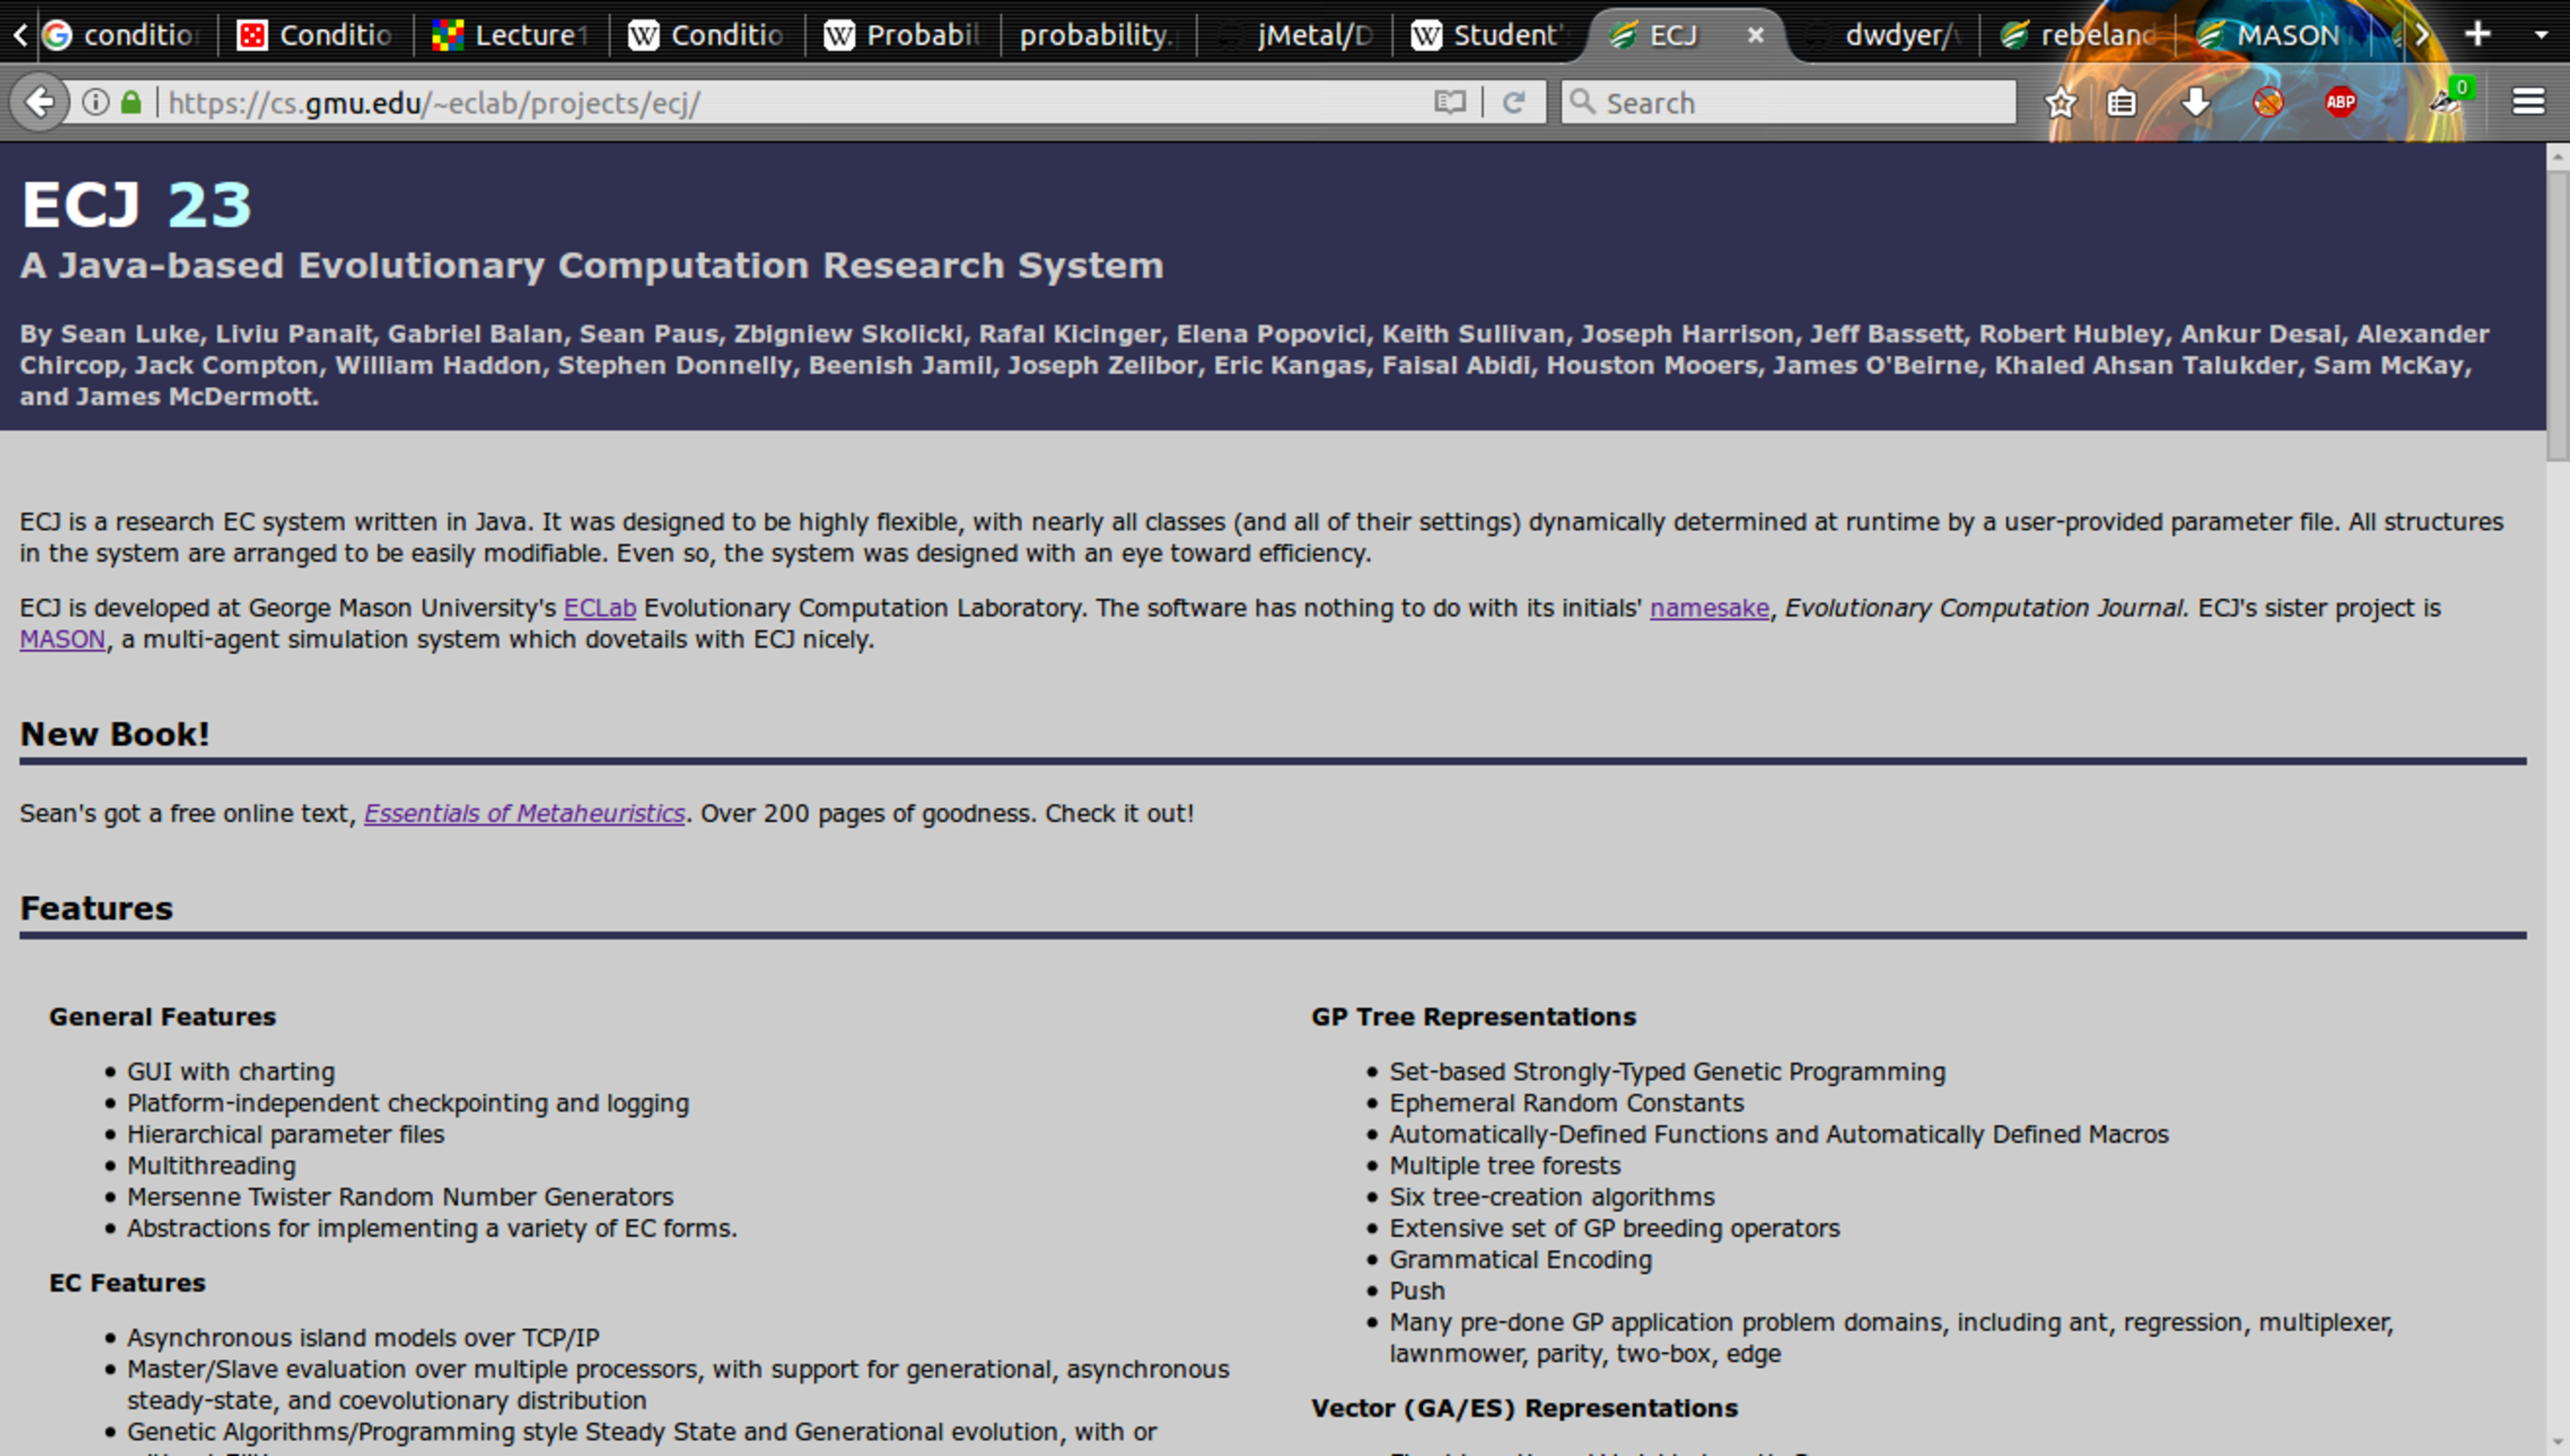
\includegraphics[width=0.9\textwidth,keepaspectratio]{ecj-url.pdf}
	\end{figure}
\end{frame}
%%
\begin{frame}
	\frametitle{Features}
	\begin{footnotesize}
	\begin{itemize}
		\item A fairly complete GP research system.
		\item Set-based GP, Strongly Typed GP, ADF, ADM, Multi-tree (forests), Tree generation algorithms, all sorts of GP operators, GE, Push, lots of examples and benchmark problem sets.
		\item Other EC Algorithms: GA, ES, DE, PSO, EMO and CMAES etc.
		\item EC models: Steady State, Island Models, Co-evolution, Massively parallel evaluation etc.
		\item All kinds of EC related operators.
		\item Fairly good collection of benchmark problems.
		\item EMO: only NSGA-II and SPEA2, ZDT and DTLZ problems, no performance measure facility.
	\end{itemize}
	\end{footnotesize}
\end{frame}
%%
\begin{frame}
	\frametitle{Why/Why not ECJ?}
	\begin{columns}[c]
		\column{1.5in}
			\begin{figure}
				\centering
				
\includegraphics[width=1.5in,keepaspectratio]{java-bug.pdf}
				\caption{Pattern in \texttt{java.util.Random}}
			\end{figure}
		\column{3in}
		\begin{scriptsize}
			\begin{itemize}
				\setlength{\itemsep}{0.30cm}
				\item No particular reason.
				\item Java random number generator (\texttt{java.util.Random}) used to have a bug (fixed in 2009). ECJ has it's own correctly implemented RNG (Mersenne Twister), very efficient and fast.
				\item Covers almost all aspects in EC in general. There are other frameworks (i.e. \textit{watchmaker}), but not as vast as ECJ.
				\item Strong emphasis on efficient code. (\(O(N^2)\) vs. \(O(\log N)\)) -- \textit{therefore, sometimes it's quite hard to understand the code, steep learning curve.}
				\item Time consuming to implement a simple concept, but very easy to do complicated experiments.
			\end{itemize}
		\end{scriptsize}
	\end{columns}
\end{frame}
%%
\begin{frame}
	\frametitle{ECJ Architecture}
	\begin{columns}[c]
		\column{2in}
			\begin{figure}
				\centering
				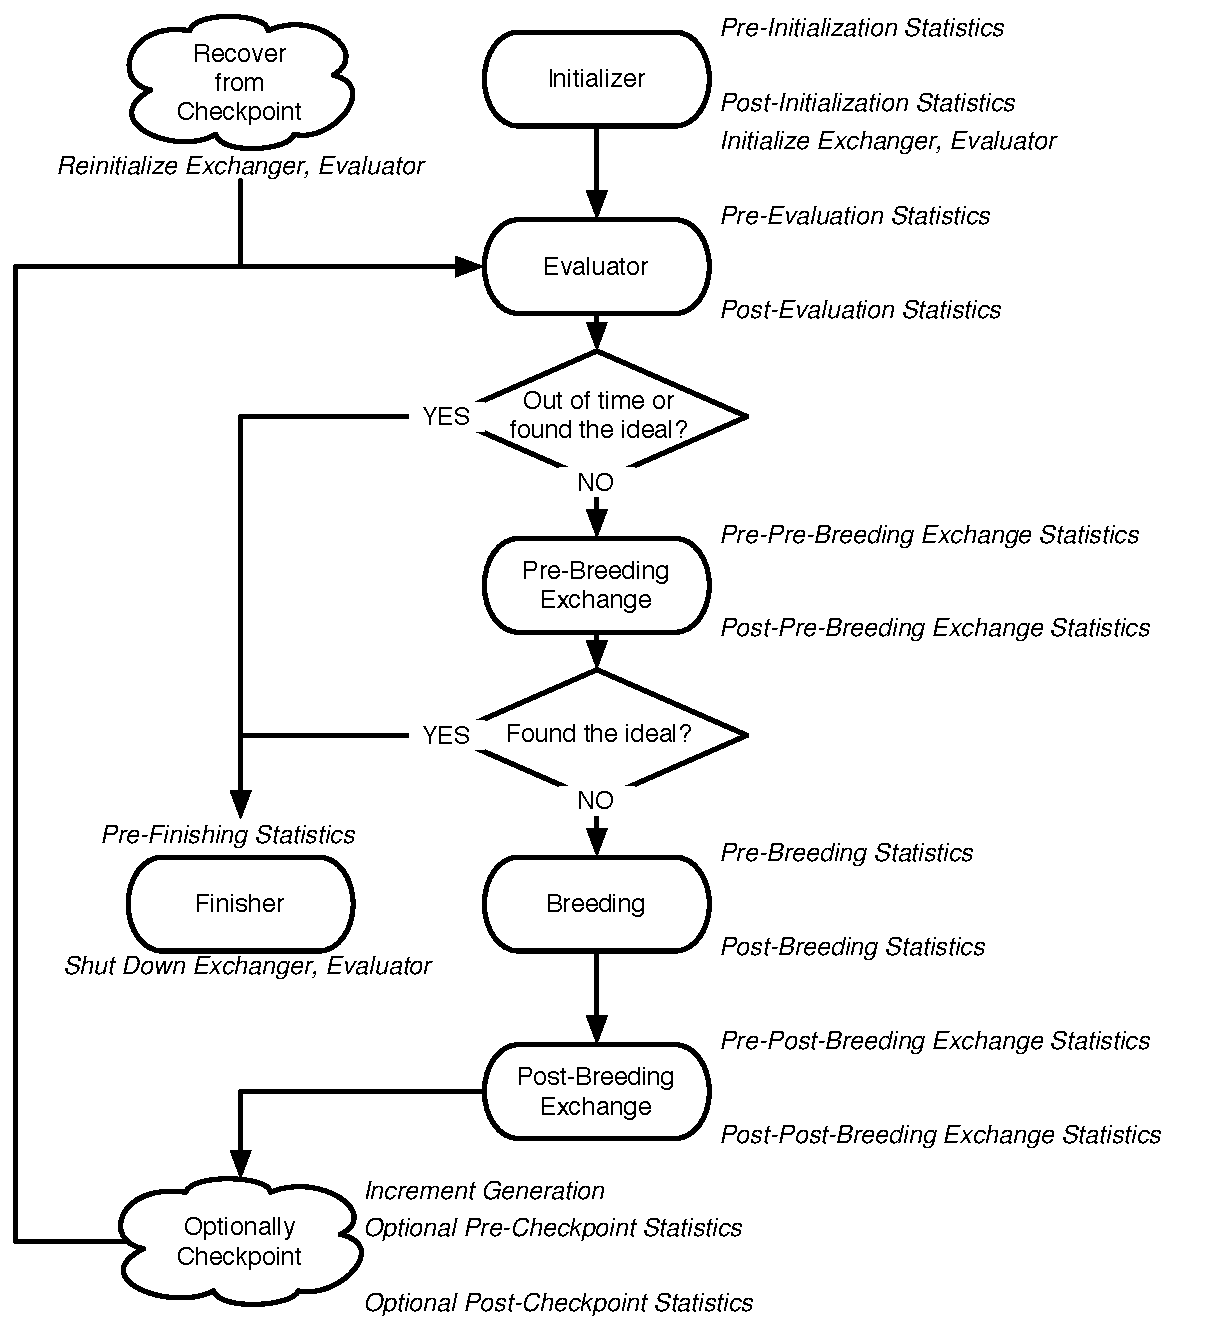
\includegraphics[width=2in,keepaspectratio]{ecj-state.pdf}
				% \caption{Pattern in \texttt{java.util.Random}}
			\end{figure}
		\column{3in}
		\begin{scriptsize}
			\begin{itemize}
				\setlength{\itemsep}{0.30cm}
				\item Everything starts from a parameter file.
				\item Example run: \texttt{java ec.Evolve -file file.params}
				\item Objects are instantiated from parameter files.
				\item Parameters can be inherited.
				\item Parameters can form hierarchies.
				\item 300 page manual: \url{https://cs.gmu.edu/~eclab/projects/ecj/docs/manual/manual.pdf}
				\item \textbf{Show an example.}
			\end{itemize}
		\end{scriptsize}
	\end{columns}
\end{frame}
%------------------------------------------------
\section{Meta-EA}	% 3
\begin{frame}
	\frametitle{An Example Experiment: Meta-EA}
	\begin{footnotesize}
	\begin{itemize}
		\item Meta-EAs: finding the best EA parameters for a particular algorithm to solve a specific problem.
		\item Digression: Given a specific FE budget, and a parallel computing resource, when it is worthwhile to run a Meta-EA? and how should we run it?
		\item Is it possible to smooth out the EA parameter space? Testing one meta-individual (EA parameter settings) multiple times or just once?
		\item Evolve the meta-individuals according to the mean fitness from multiple test.
		\item Look for the strategy that will most likely to give the best solution to a particular problem.
		\item Massively parallel evaluation implemented using ECJ to run over a 128 node cluster, \textbf{14.2 million evolutionary runs} for different EAs and benchmark problems.
	\end{itemize}
	\end{footnotesize}
\end{frame}
%
\begin{frame}
	\frametitle{Meta-EA: Sample Result}
	\begin{columns}[c]
		\column{2.5in}
			\begin{figure}
				\centering
				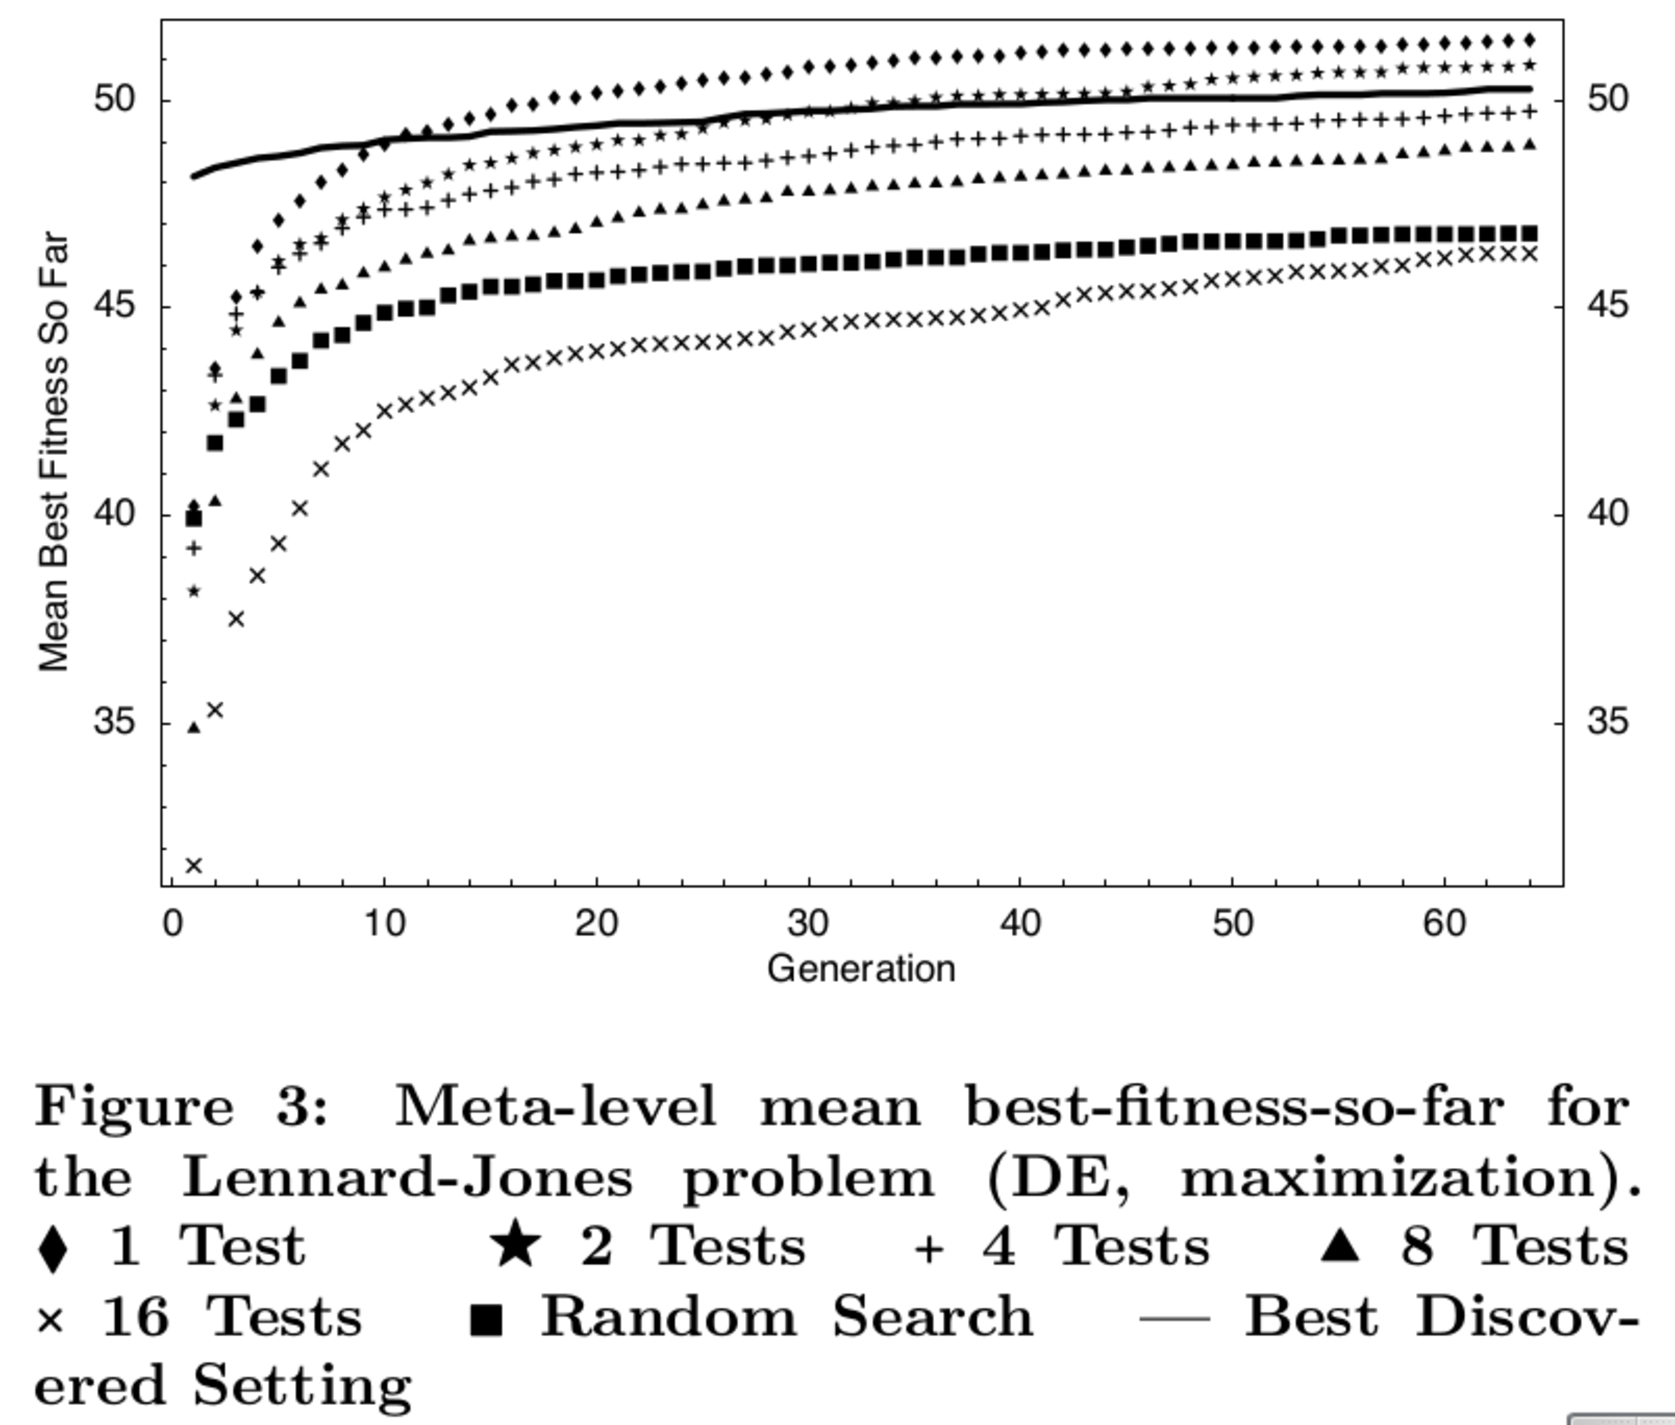
\includegraphics[width=2.5in,keepaspectratio]{meta-ea.pdf}
				% \caption{Pattern in \texttt{java.util.Random}}
			\end{figure}
		\column{2.5in}
		\begin{scriptsize}
			\begin{itemize}
				\setlength{\itemsep}{0.30cm}
					\item Turns out that smoothing of the parameter space is not very useful if the budget is fixed.
					\item Specific example: 1, 2, 4, 8, 16 tests vs. 128, 64, 32, 16, 8 meta level pop. size.
					\item It's better to try 128 different parameter settings once than 8 parameter settings 8 times to get the ``best solution discovering'' parameter.
			\end{itemize}
		\end{scriptsize}
	\end{columns}
\end{frame}
%------------------------------------------------
\section{MASON}		% 2
\begin{frame}
	\frametitle{MASON: \textbf{M}ulti-\textbf{A}gent \textbf{S}imulator of \textbf{N}eighborhoods\(\ldots\)\\or \textbf{N}etworks\(\ldots\) or something\(\ldots\)}
	\begin{itemize}
		\item Fast discrete event simulator developed at GMU Autonomous Robotics Lab and Center for Social Complexity, Krasnow Institute of Advanced Studies.
		\item Initial objective was to do black-box simulation optimization with ECJ, but later came out as an independent project.
		\item More popular than ECJ, especially in the simulation science community.
		\item Also written in Java.
	\end{itemize}
\end{frame}
%%
\begin{frame}
	\frametitle{MASON: \textbf{M}ulti-\textbf{A}gent \textbf{S}imulator of \textbf{N}eighborhoods\(\ldots\)\\or \textbf{N}etworks\(\ldots\) or something\(\ldots\)}
	\begin{figure}
		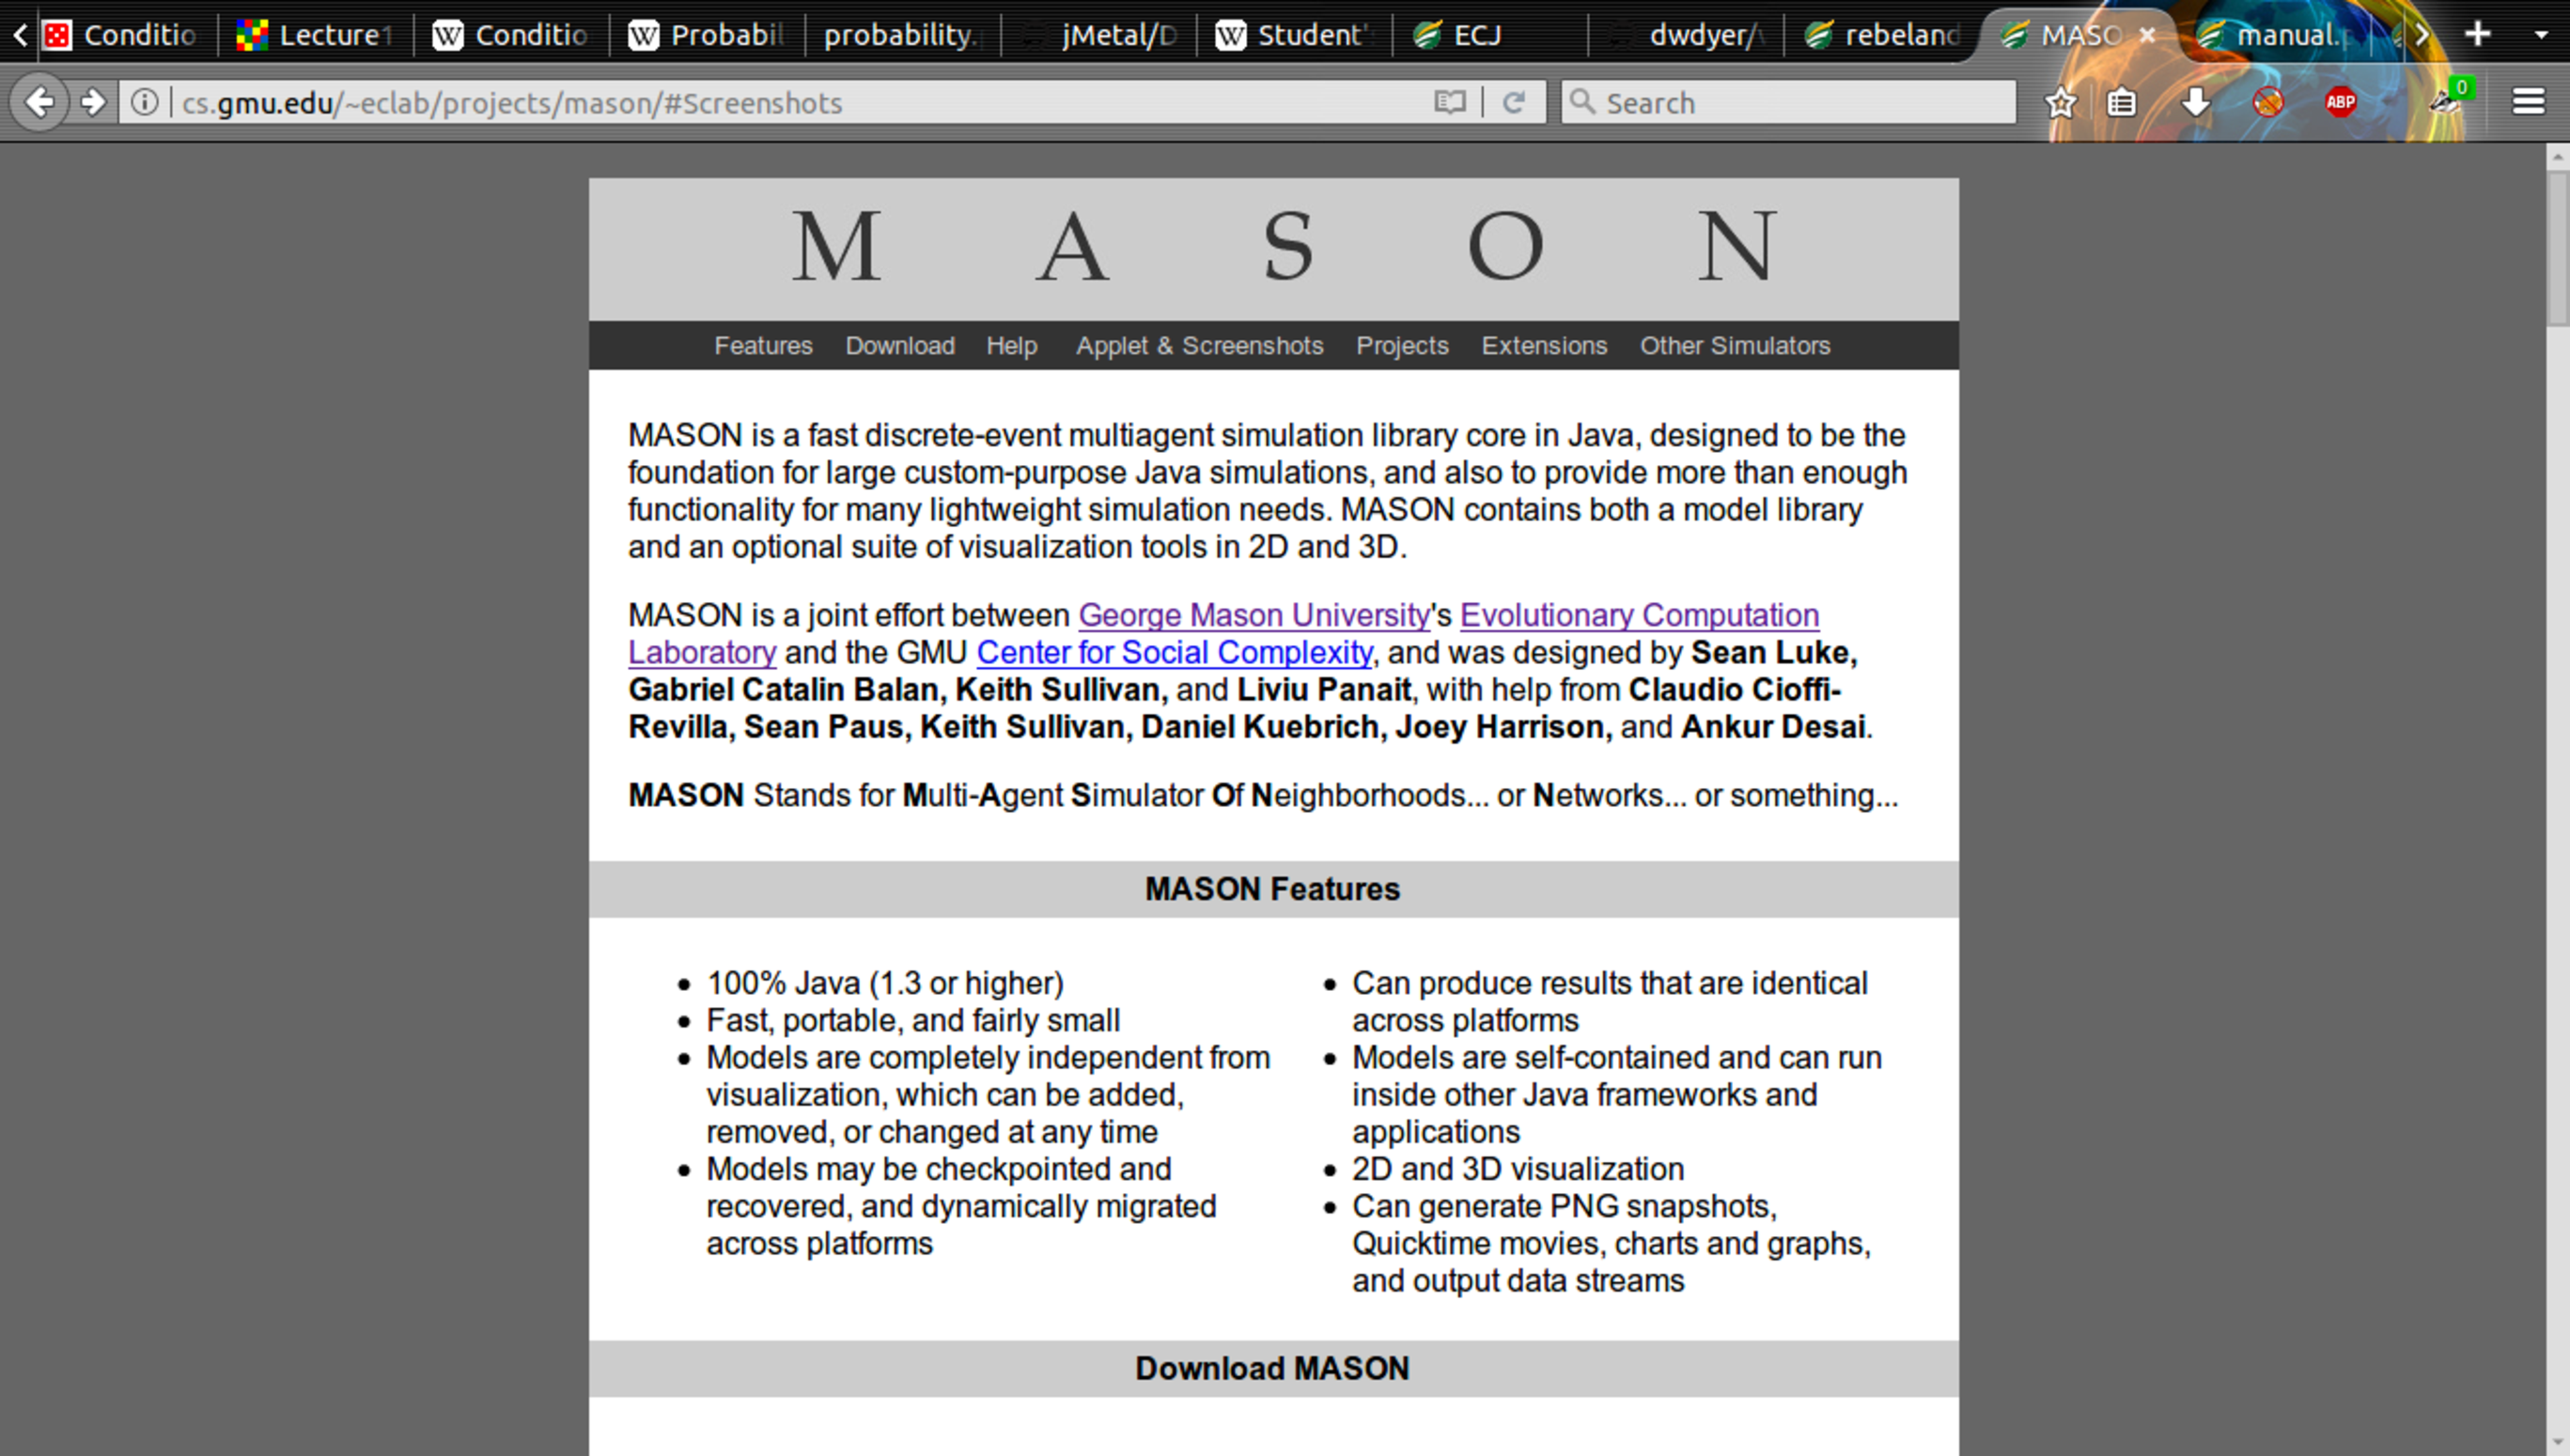
\includegraphics[width=0.8\textwidth,keepaspectratio]{mason-url.pdf}
	\end{figure}
\end{frame}
%%
\begin{frame}
	\frametitle{Features}
	\begin{footnotesize}
	\begin{itemize}
		\item Can represent continuous, discrete, or hexagonal 2D, 3D, or Network data, and any combination of it.  
		\item Full-fledge GUI for visualization, probing and monitoring simulation activities.
		\item The Console gives access to model data, plays, stops, pauses, and steps the simulation, checkpoints and recovers models, and performs other tasks.  
		\item The user can also view and change per-object model data by selecting objects in the visualization displays and bringing up their inspectors.
		\item Very fast and efficiently written (like ECJ)
		\item It also comes with a 300 page manual (\url{http://cs.gmu.edu/~eclab/projects/mason/manual.pdf})
	\end{itemize}
	\end{footnotesize}
\end{frame}
%%
\begin{frame}
	\frametitle{Examples}
	\begin{figure}
		\vspace{-20pt}
		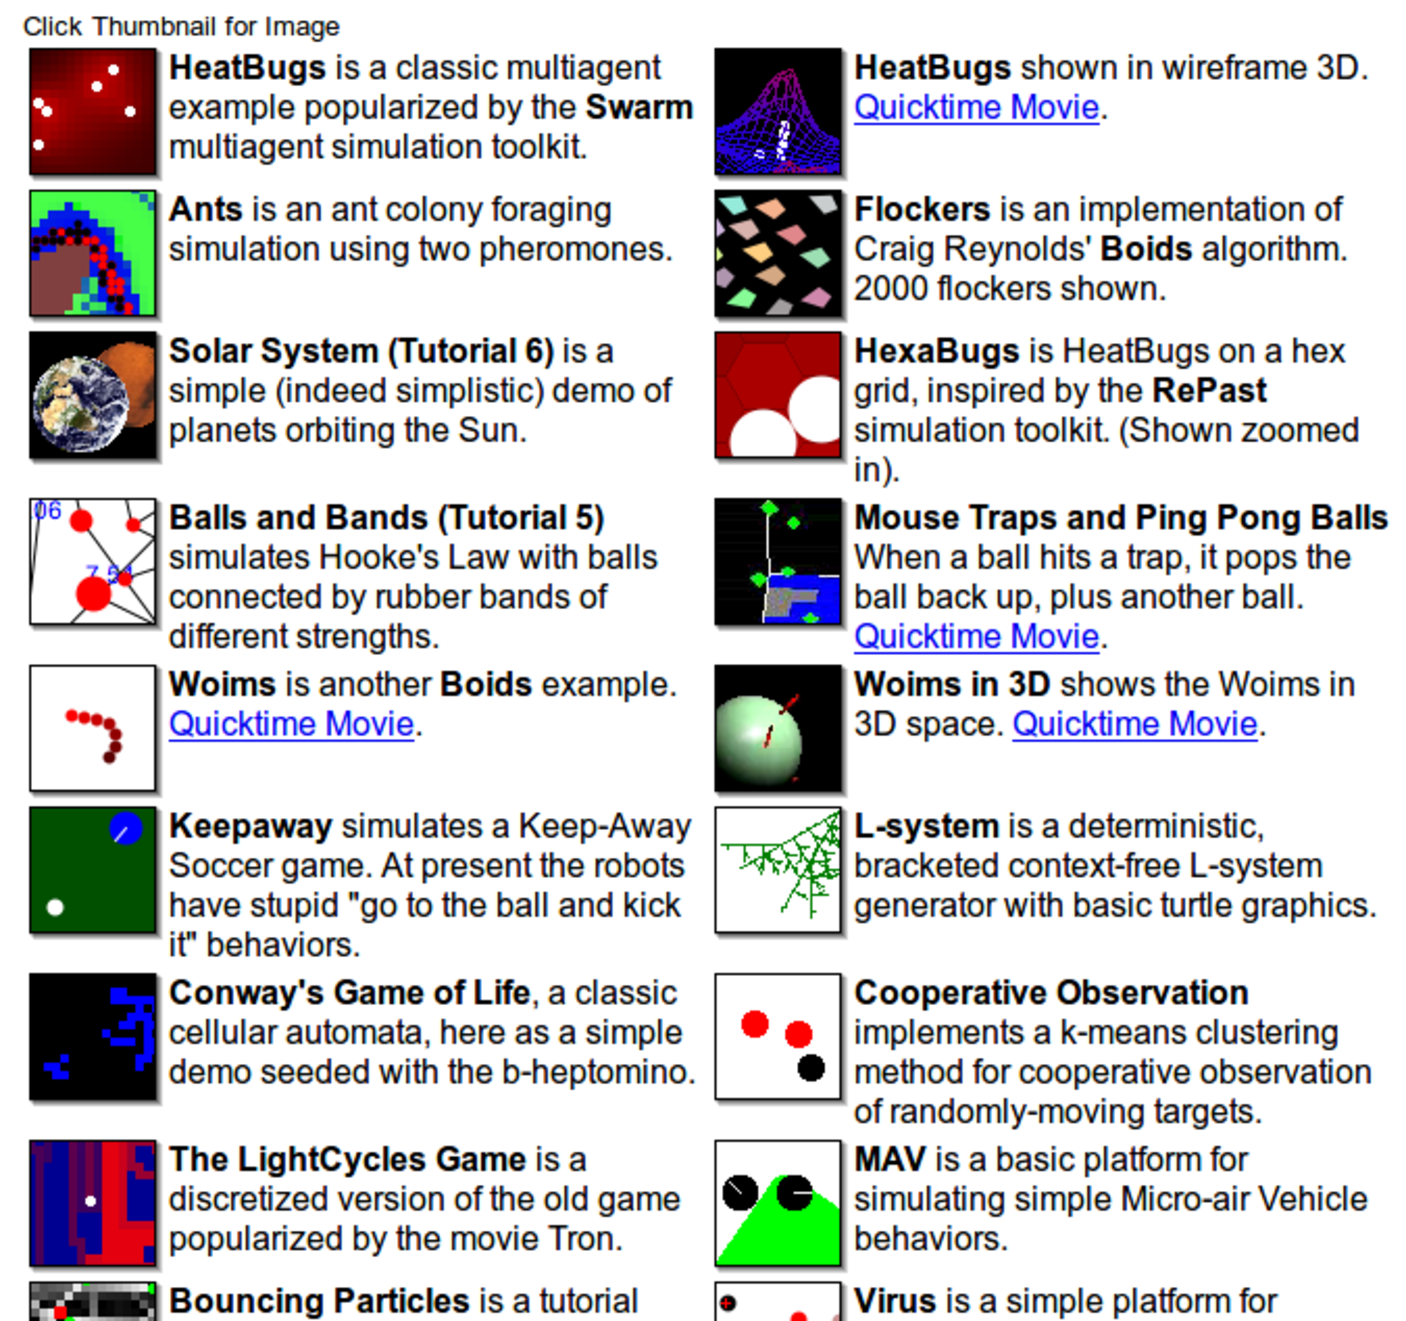
\includegraphics[width=0.65\textwidth,keepaspectratio]{mason-applet.pdf}
	\end{figure}
\end{frame}
%------------------------------------------------
% \section{HiTAB}		% 2
% \begin{frame}
% 	\frametitle{HiTAB: Hierarchical Training of Agent Behavior}
% \end{frame}
%------------------------------------------------
\section{MASON + ECJ}	% 1
\begin{frame}
	\frametitle{Gluing ECJ with MASON}
	\begin{columns}[c]
	\column{2in}
		\centering
		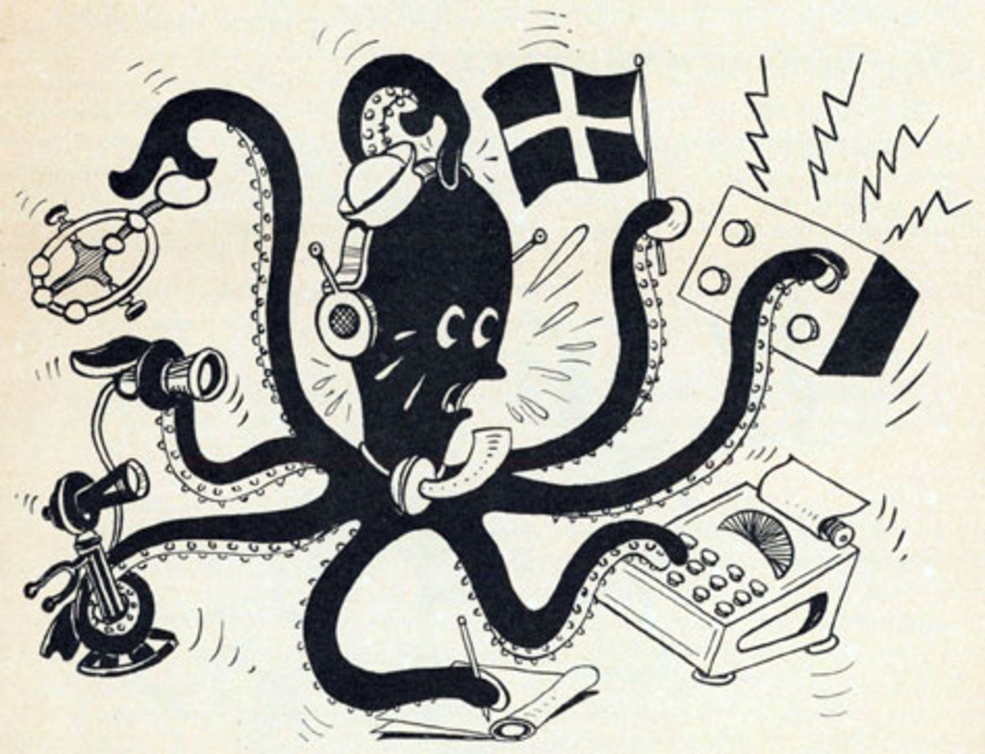
\includegraphics[width=2in,keepaspectratio]{octopus.pdf}
	\column{2.5in}
		%\begin{scriptsize}
			\begin{itemize}
			\setlength{\itemsep}{15pt}
				\item Scientists make \textbf{models}.
				\item Complicated models (i.e. ABM) requires a large number of \textbf{multiple inter-dependent parameters} to be tuned manually -- prohibitive.
				\item \textbf{Can we automate this ?}
			\end{itemize}
		%\end{scriptsize}
	\end{columns}
\end{frame}
%%
\begin{frame}
	\frametitle{Preliminaries}
	\begin{block}{Model Parameter Types}
		\begin{scriptsize}
			\begin{itemize}
				\item Known Parameters -- whose settings already known for a fact
				\item Inferable Parameters -- whose settings should be set in a certain way \\(\emph{according to a particular theory})
				\item Insensitive Parameters -- over whose settings the model is expected to be insensitive
				\item \textbf{Unknown Parameters -- on which an experimenter has no idea/control over.}\\ (\emph{most interesting ?})
			\end{itemize}
		\end{scriptsize}
	\end{block}
	\vspace{-10pt}
	\begin{block}{Goals}
		\begin{footnotesize}
			\begin{itemize}
				\item To produce a certain kind of output which is predicted by a theory, or 
				\item to match and validate against known real-world results.
			\end{itemize}
		\end{footnotesize}
	\end{block}
\end{frame}
%%
\begin{frame}
	\frametitle{Parallel Evolutionary Optimization -- A Bird's-Eye View}
	\begin{columns}[c]
	\column{2in}
		%\begin{small}
			\begin{itemize}
			\setlength{\itemsep}{20pt}
				\item Extremely expensive -- need to optimize the model by running it many times.
				\item Ought to be done in parallel.	
			\end{itemize}
		%\end{small}
	\column{3in}
		\centering
		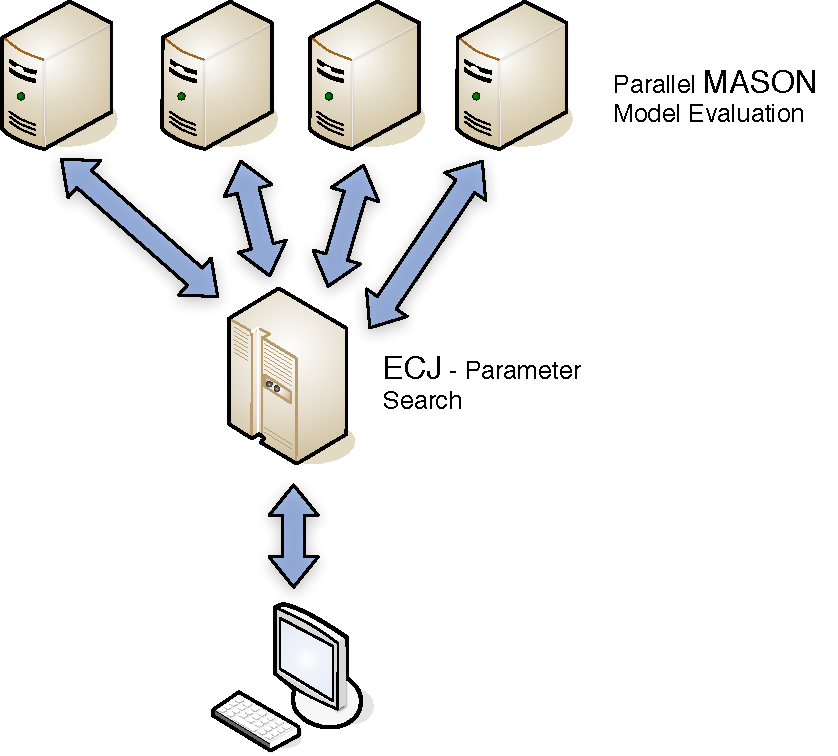
\includegraphics[width=2.5in,keepaspectratio]{master-slave.pdf}	
	\end{columns}
\end{frame}
%------------------------------------------------
\section{PacMan}	% 3
\begin{frame}
	\frametitle{A Very Simple GP Experiment: Evolving PacMan Behavior}
	\begin{block}{}
		\begin{itemize}
			\setlength{\itemsep}{0.75cm}
			\item MASON $\rightarrow$ \textbf{Behaviour} specifications
			\item ECJ $\rightarrow$ \textbf{Optimization} by \textbf{Evolution}
			\item MASON $+$ ECJ $\rightarrow$ Evolving Optimized Behaviour
			\item \textbf{Target}: The game of PacMan 
		\end{itemize}
	\end{block}
\end{frame}
%%
\begin{frame}
	\frametitle{An Evolved Pac Behaviour}
	\begin{block}{}
		\centering
		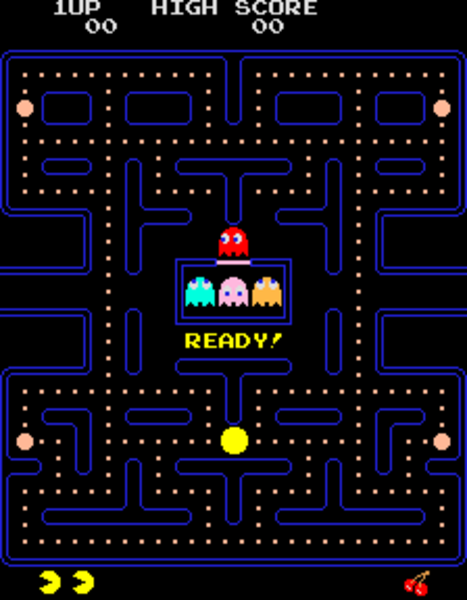
\includegraphics[width=1.5in,keepaspectratio]{pac-man.pdf}
	\end{block}
	\vspace{-25pt}
	\begin{block}{}
		\Huge{\centerline{Show Demo}}
	\end{block}
\end{frame}
%------------------------------------------------
\section{Rebeland}	% 3
\begin{frame}
	\frametitle{A More Sophisticated Example: RebeLand}
	\begin{footnotesize}
	\begin{itemize}
		\item Built on top of MASON to simulate socio-economic instability.
		\item Developed by the Center for Social Complexity, Krasnow Institute of Advanced Study, GMU
			and Smithsonian Institution.
		\item Simulate a government policies according to canonical political science and theory from
			economics
		\item Experimenter can start the simulation with a set of initial parameters and check the validity of a theory by gathering the statistical information from the simulation agents.
		\item Includes historical and geoglogical data to model resources for the population.
	\end{itemize}
	\end{footnotesize}
\end{frame}
%%
\begin{frame}
	\frametitle{RebeLand Model}
	\begin{columns}[c]
	\column{2.5in}
		\centering
		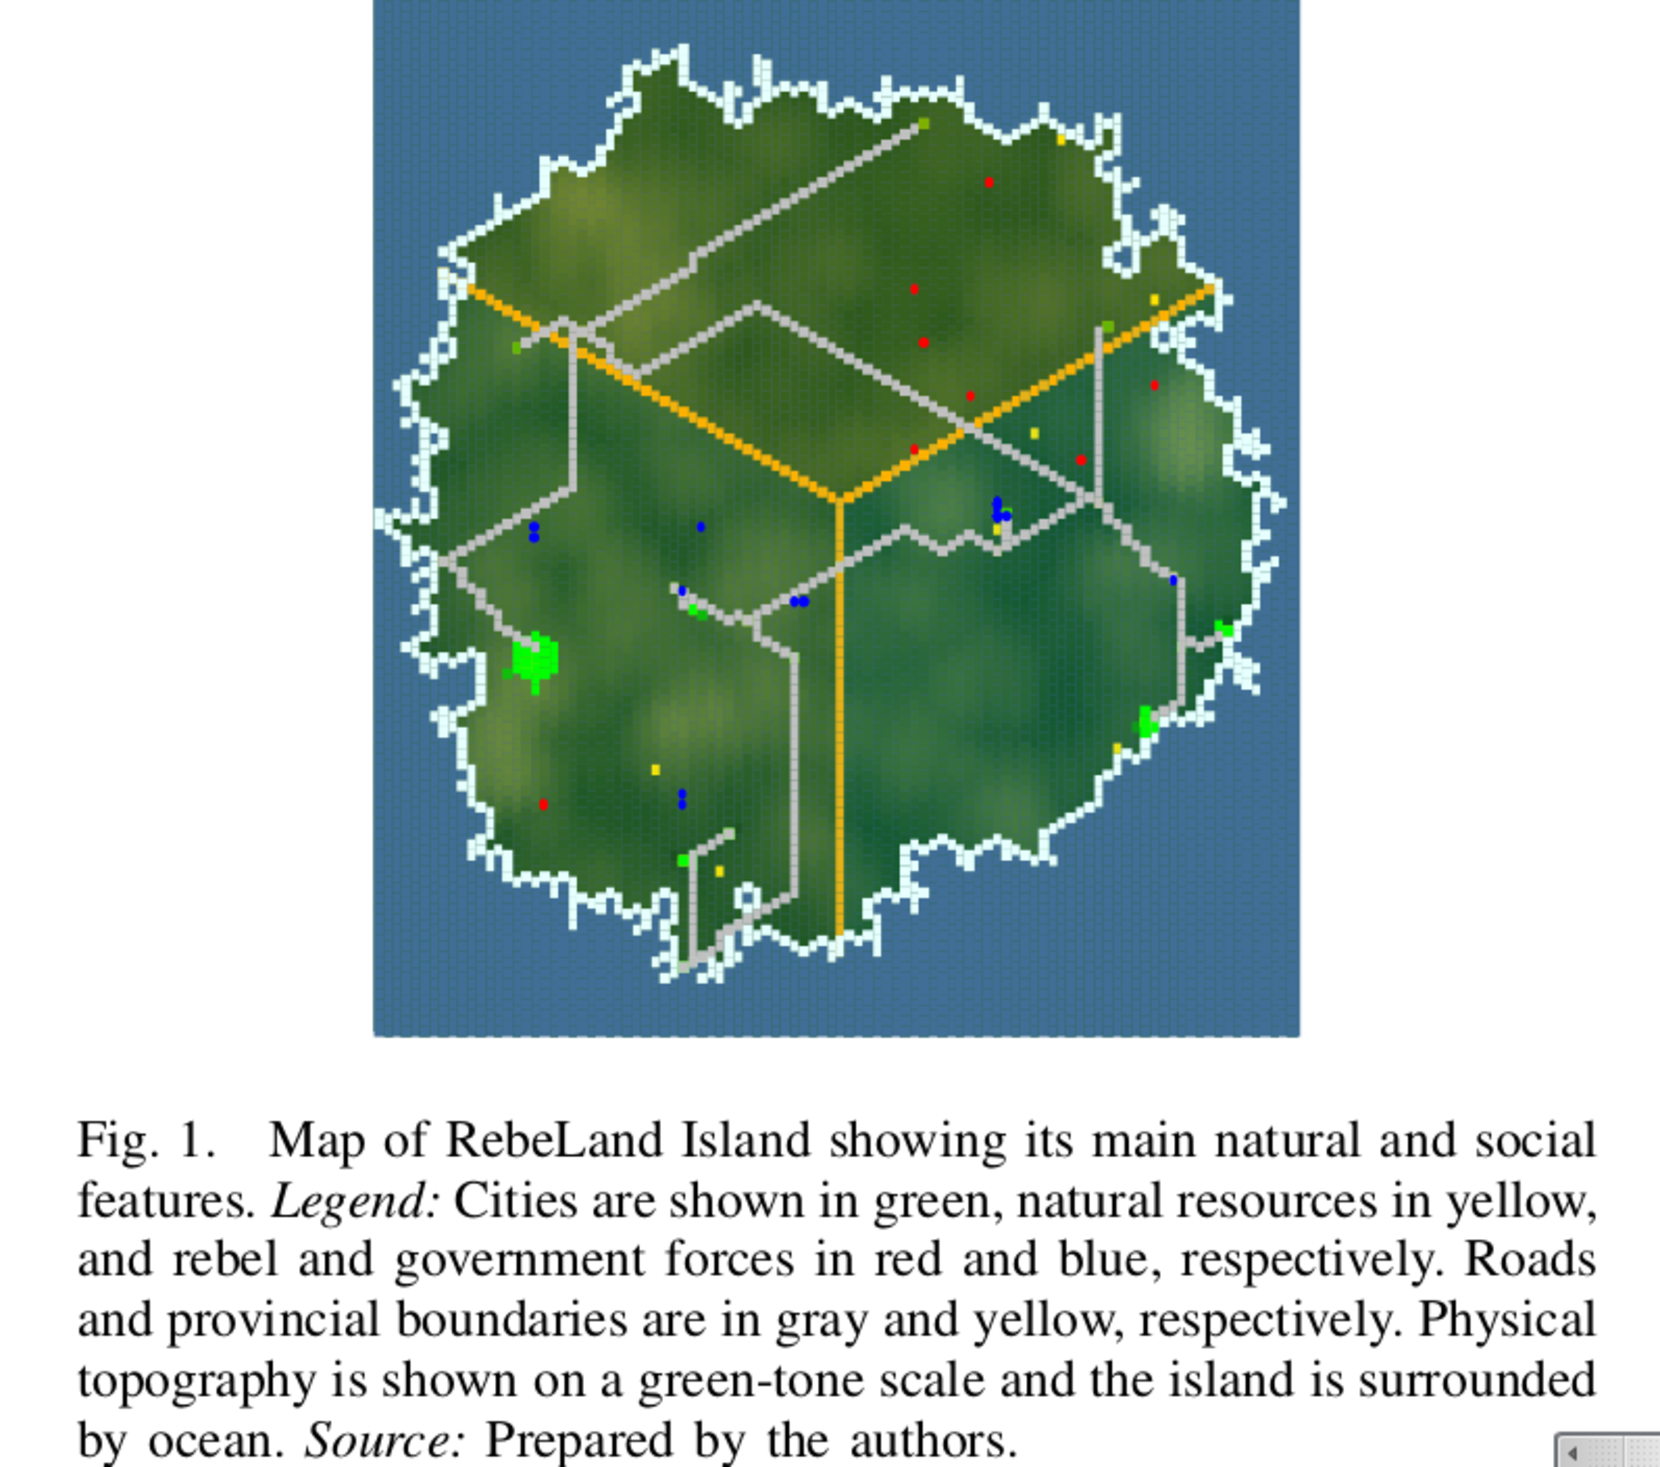
\includegraphics[width=2.5in,keepaspectratio]{rebeland-map.pdf}	
	\column{2.5in}
		\centering
		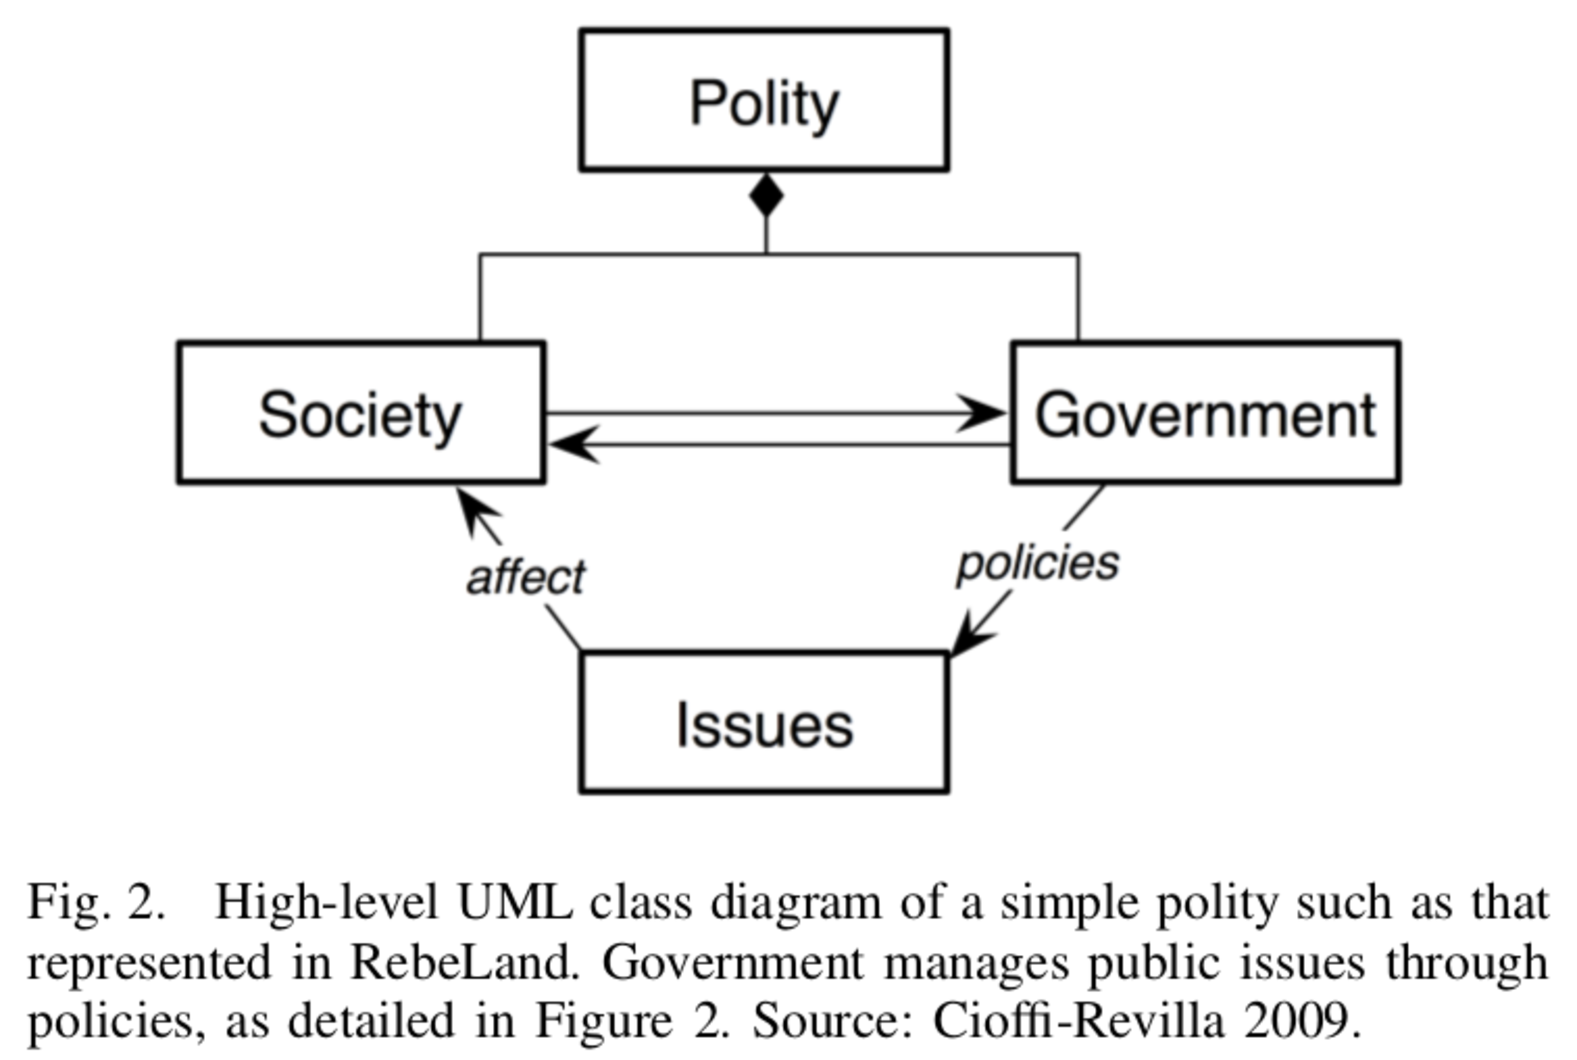
\includegraphics[width=2.5in,keepaspectratio]{rebeland-uml.pdf}	
	\end{columns}
\end{frame}
%%
\begin{frame}
	\frametitle{RebeLand Simulation Snapshot 1}
	\begin{columns}[c]
	\column{2.5in}
		\centering
		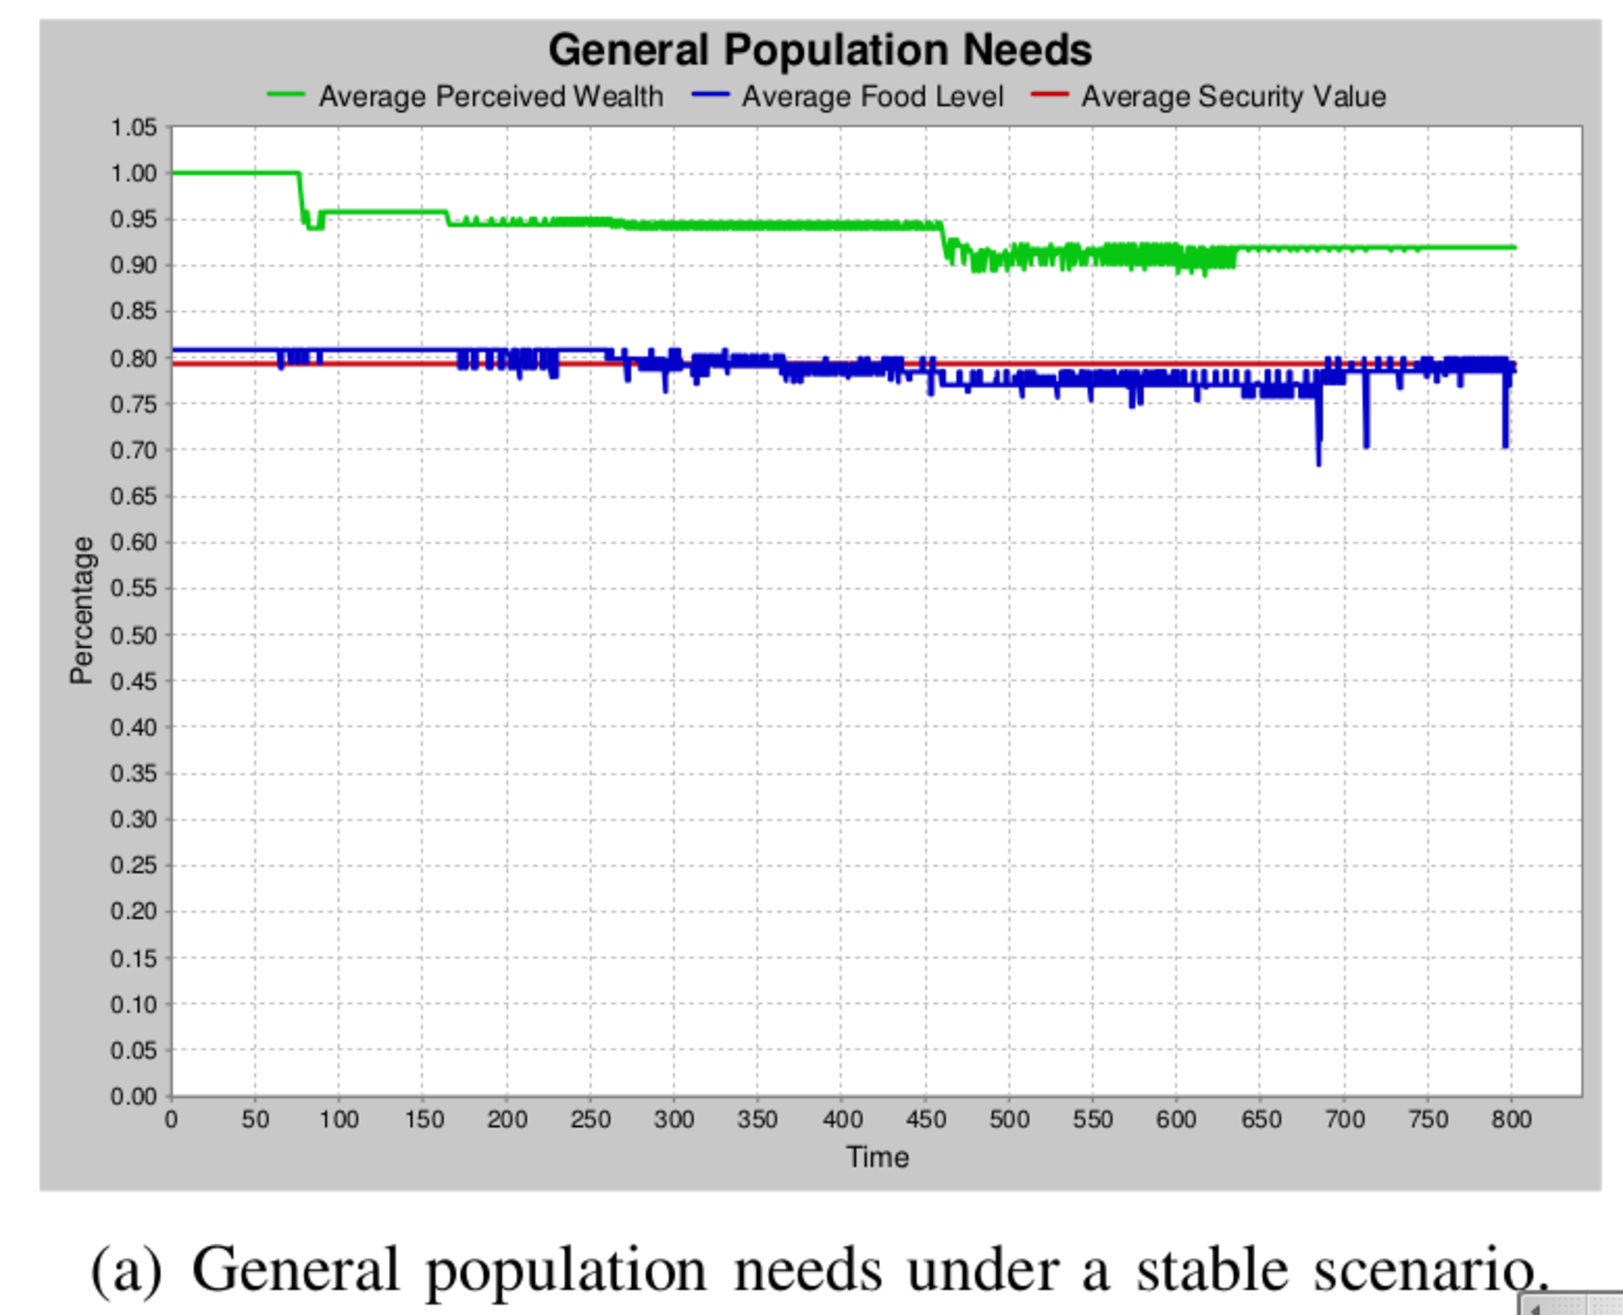
\includegraphics[width=2.5in,keepaspectratio]{population-need-stable.pdf}	
	\column{2.5in}
		\centering
		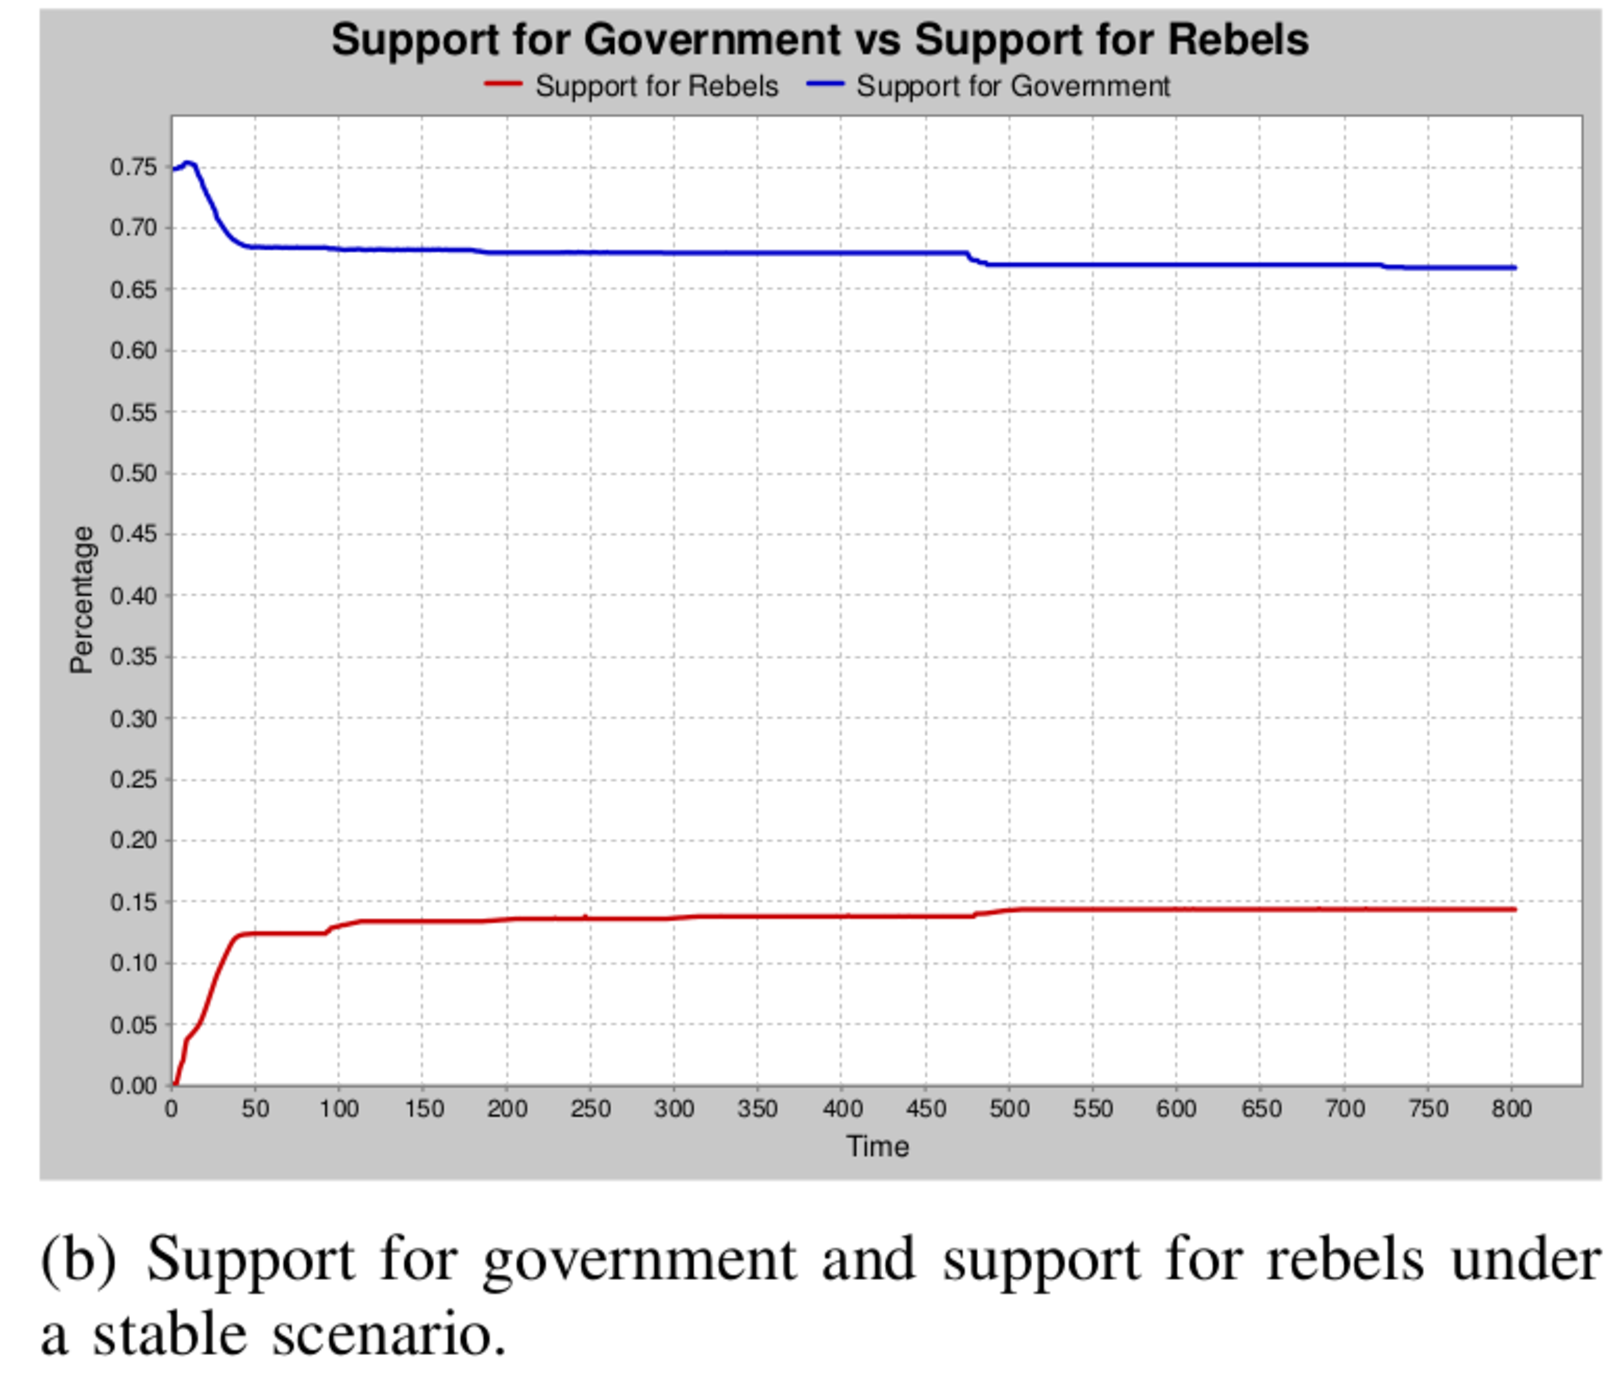
\includegraphics[width=2.5in,keepaspectratio]{support-stable.pdf}	
	\end{columns}
\end{frame}
%%
\begin{frame}
	\frametitle{RebeLand Simulation Snapshot 2}
	\begin{columns}[c]
	\column{2.5in}
		\centering
		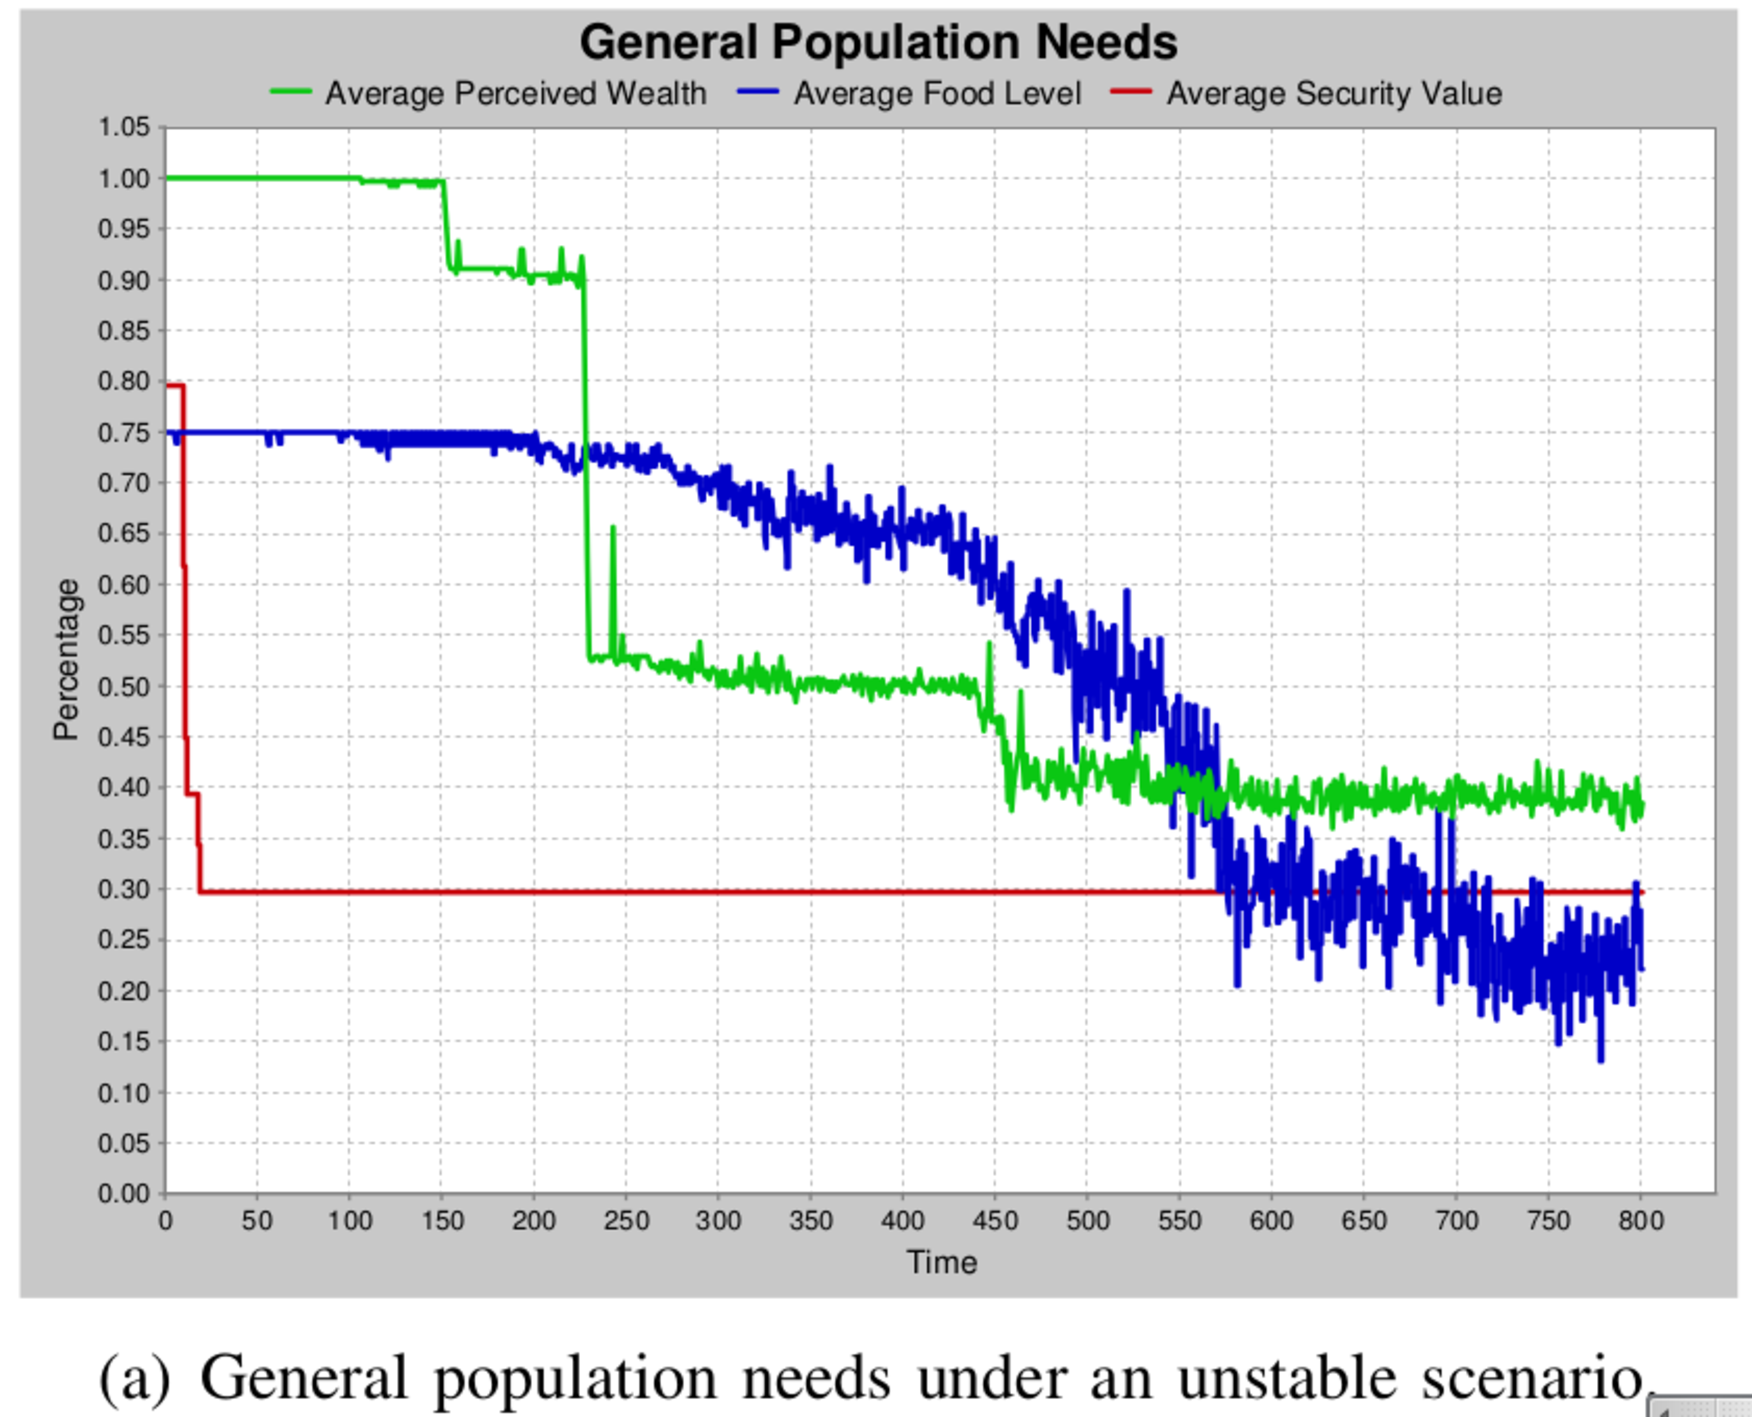
\includegraphics[width=2.5in,keepaspectratio]{population-need-unstable.pdf}	
	\column{2.5in}
		\centering
		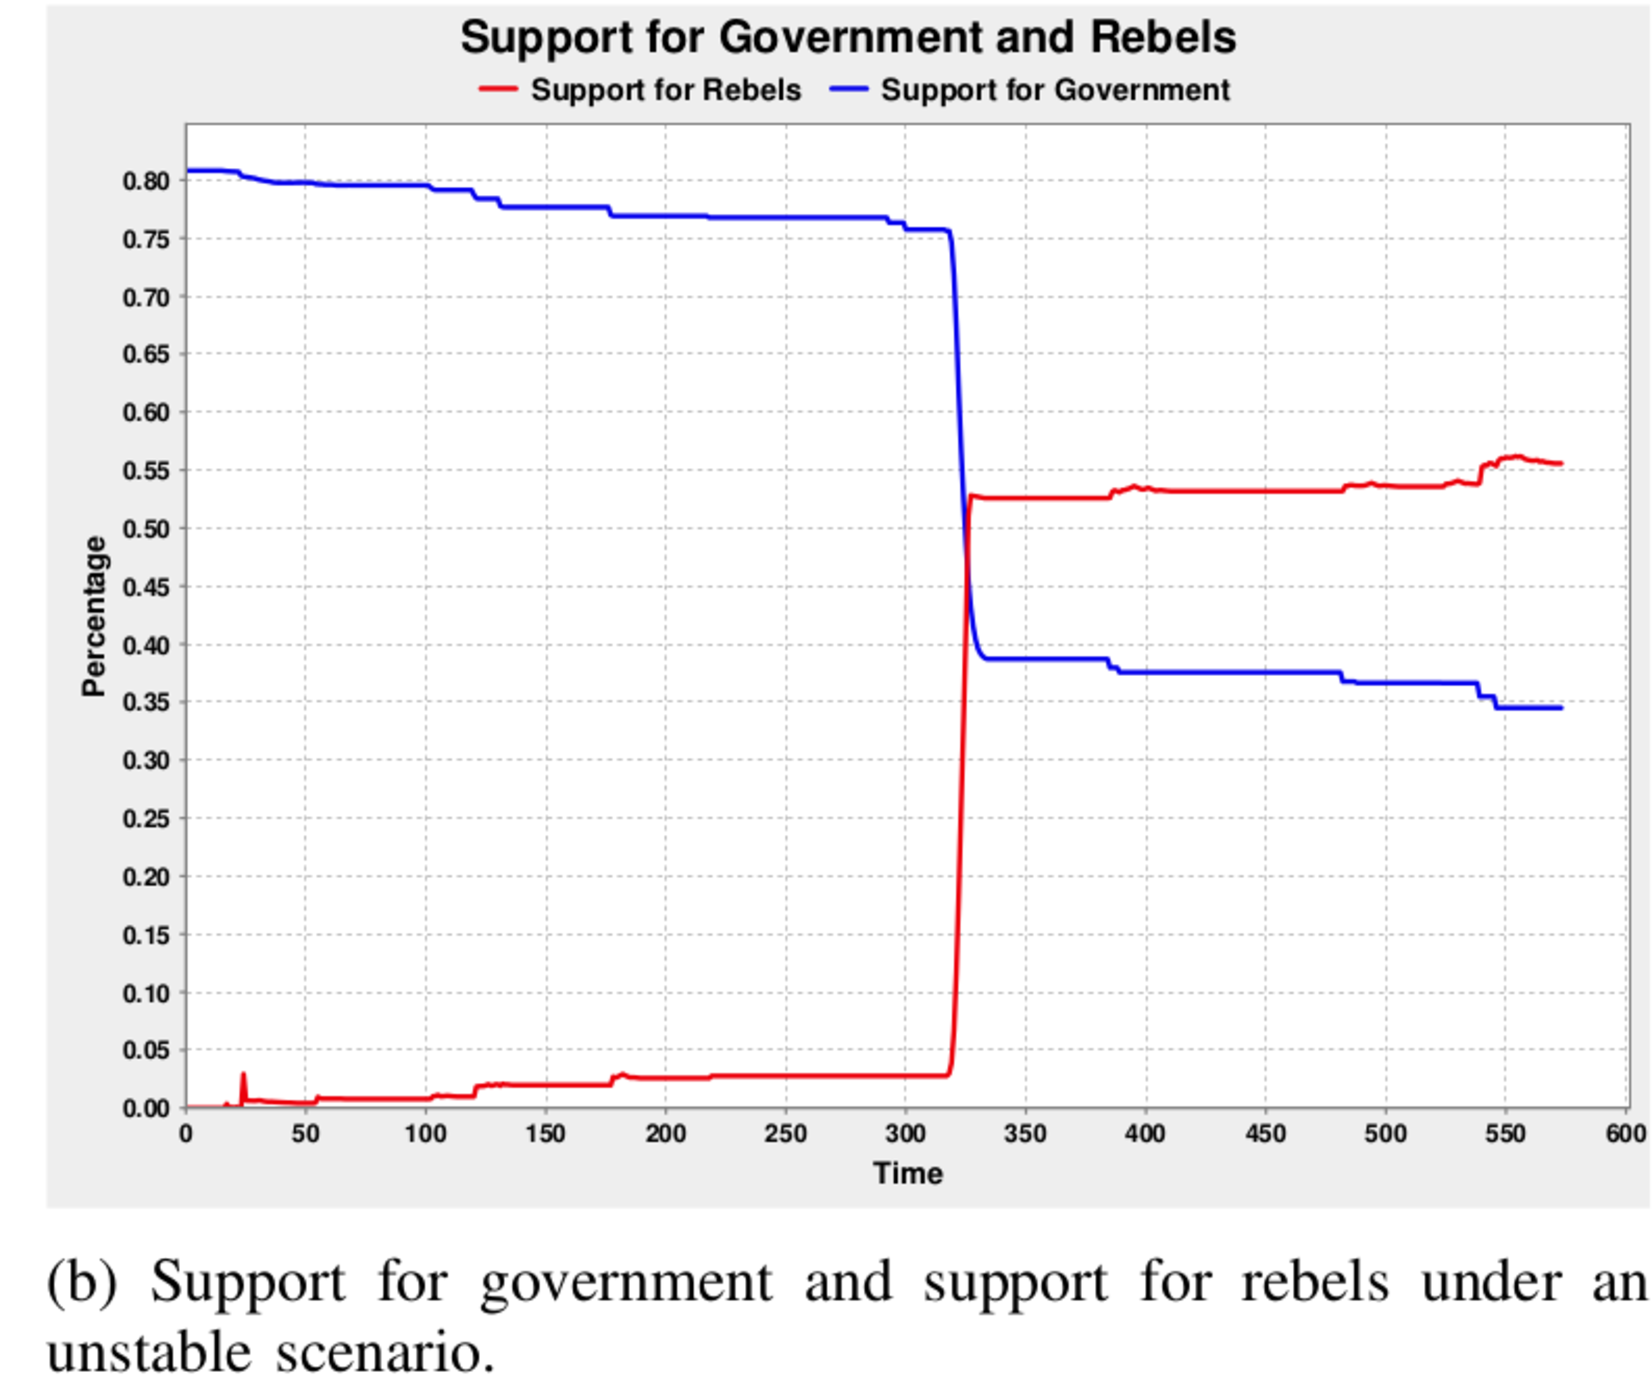
\includegraphics[width=2.5in,keepaspectratio]{support-unstable.pdf}	
	\end{columns}
\end{frame}
%%
\begin{frame}
	\frametitle{Parameters/Knobs}
	\begin{block}{Unknown Parameters to Set (\emph{all scaled to 0...1})}
		 \begin{itemize}
			\item State Corruption Rate
			\item State Tax Rate
			\item Maximum State Reserve
			\item Minimum State Reserve
			\item Minimum Spending on Populace
			\item Maximum Police Per Capita
			\item Initial Reserve Army Ratio
			\item Standing Army Size
			\item State Attack Interval
		 \end{itemize}
	\end{block}
\end{frame}
%%
\begin{frame}
	\frametitle{Details You Don't Care About}
	\begin{block}{Optimization Algorithm}
		NSGA-II, 6000 evaluations.
	\end{block}
	\begin{block}{Testing (i.e. \textit{Generalization})}
		Individual \textit{Parameter Settings} are tested by running RebeLand on MASON 8 times -- mean results were considered.
	\end{block}
	\begin{block}{Parallelization}
		Master-Slave Evaluation, 30 Slave Units on Hydra\\
		Total evaluation time: about 1 hour
	\end{block}
\end{frame}
%%
\begin{frame}
	\frametitle{Results: The \emph{Pareto Front}}
	\centering
	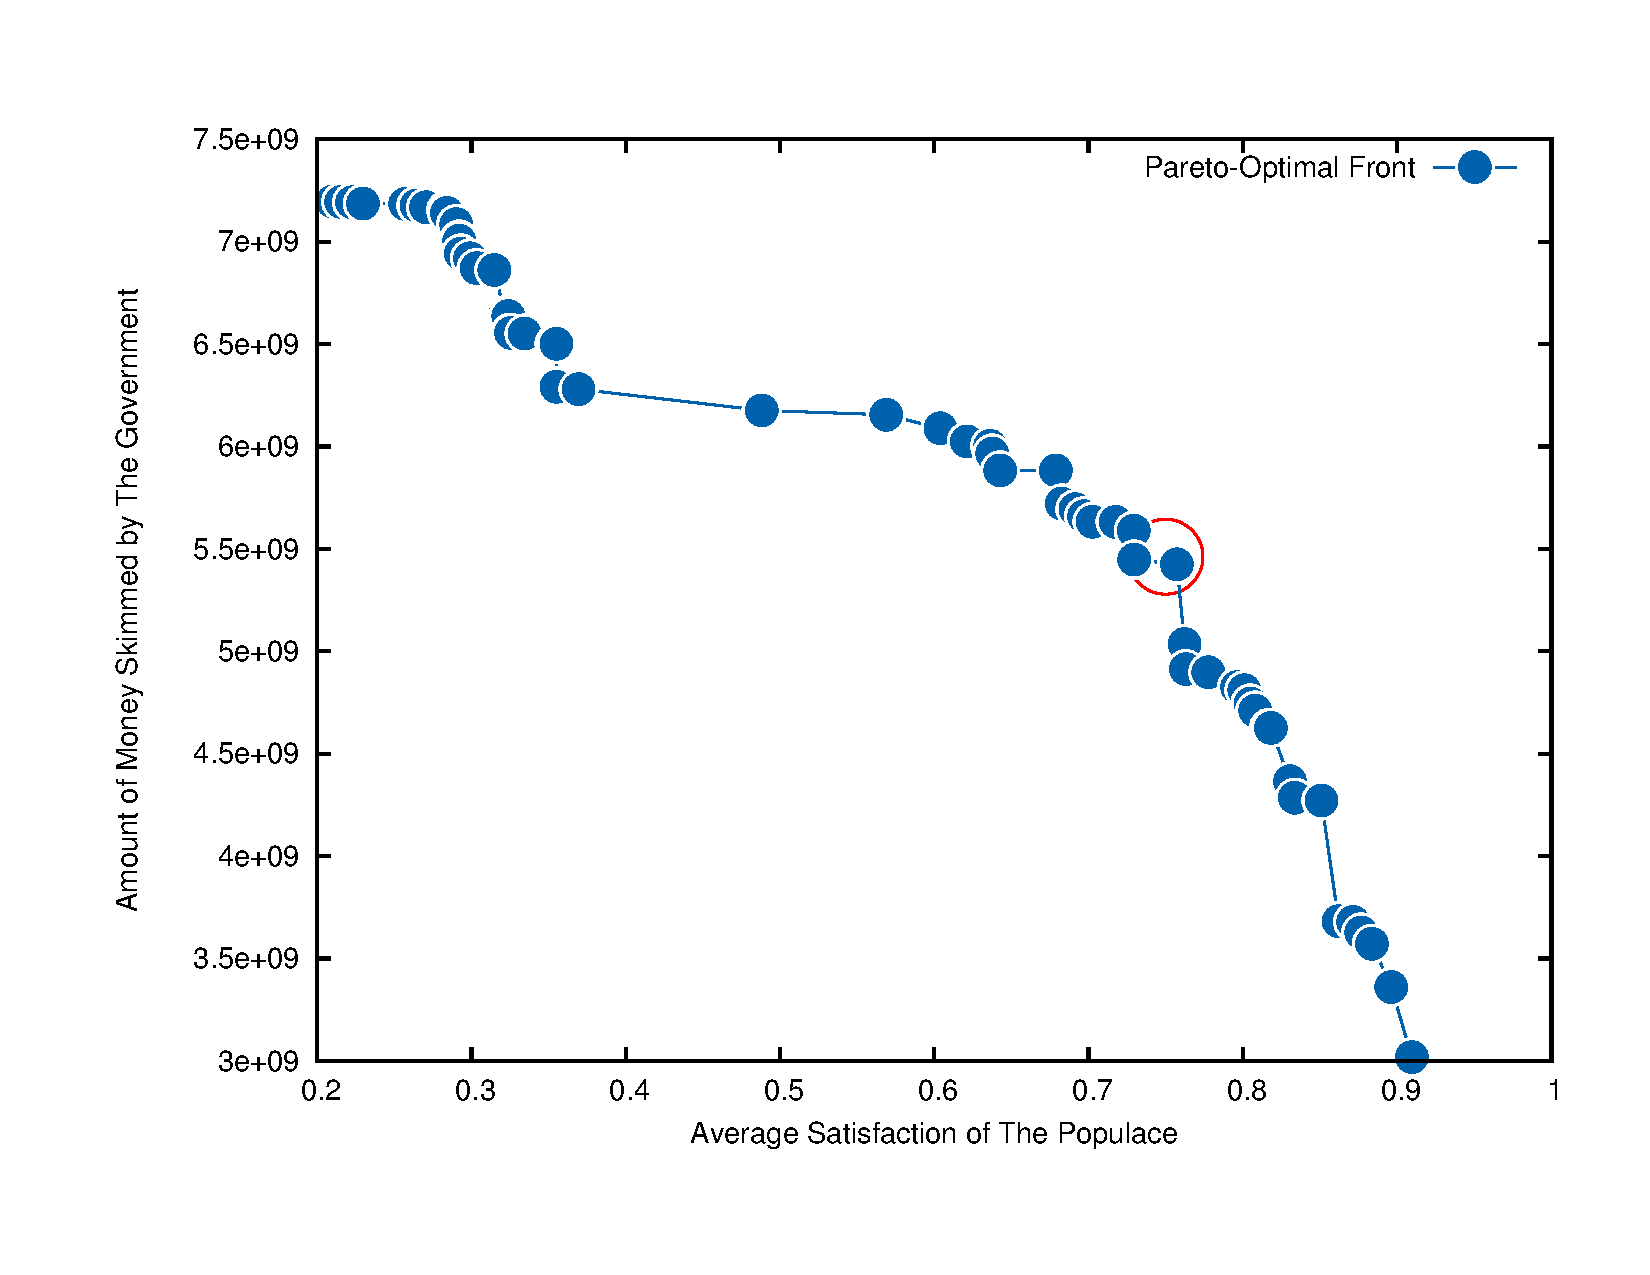
\includegraphics[width=0.8\textwidth,keepaspectratio,angle=0]{front.pdf}
\end{frame}
%%
\begin{frame}
	\frametitle{Results: Population Satisfaction}
	\begin{columns}[c]
	\column{2.5in}
		\centering
		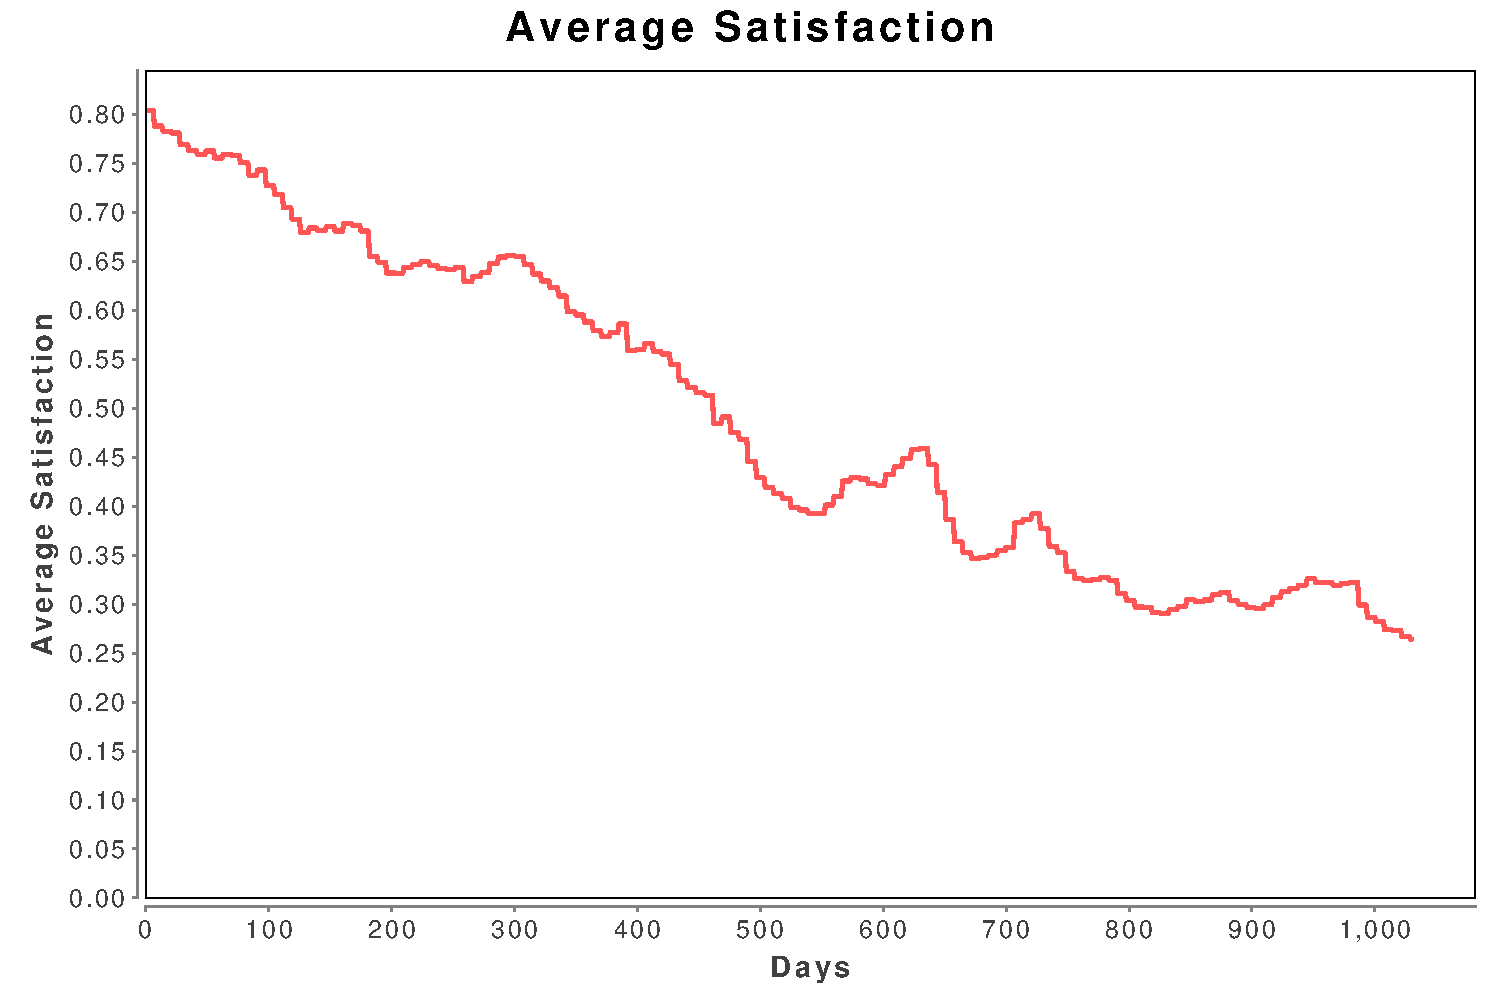
\includegraphics[width=2.25in,keepaspectratio]{average-satisfaction-old.pdf}\\
		Before Optimzation \\(Original Parameters)
	\column{2.5in}
		\centering
		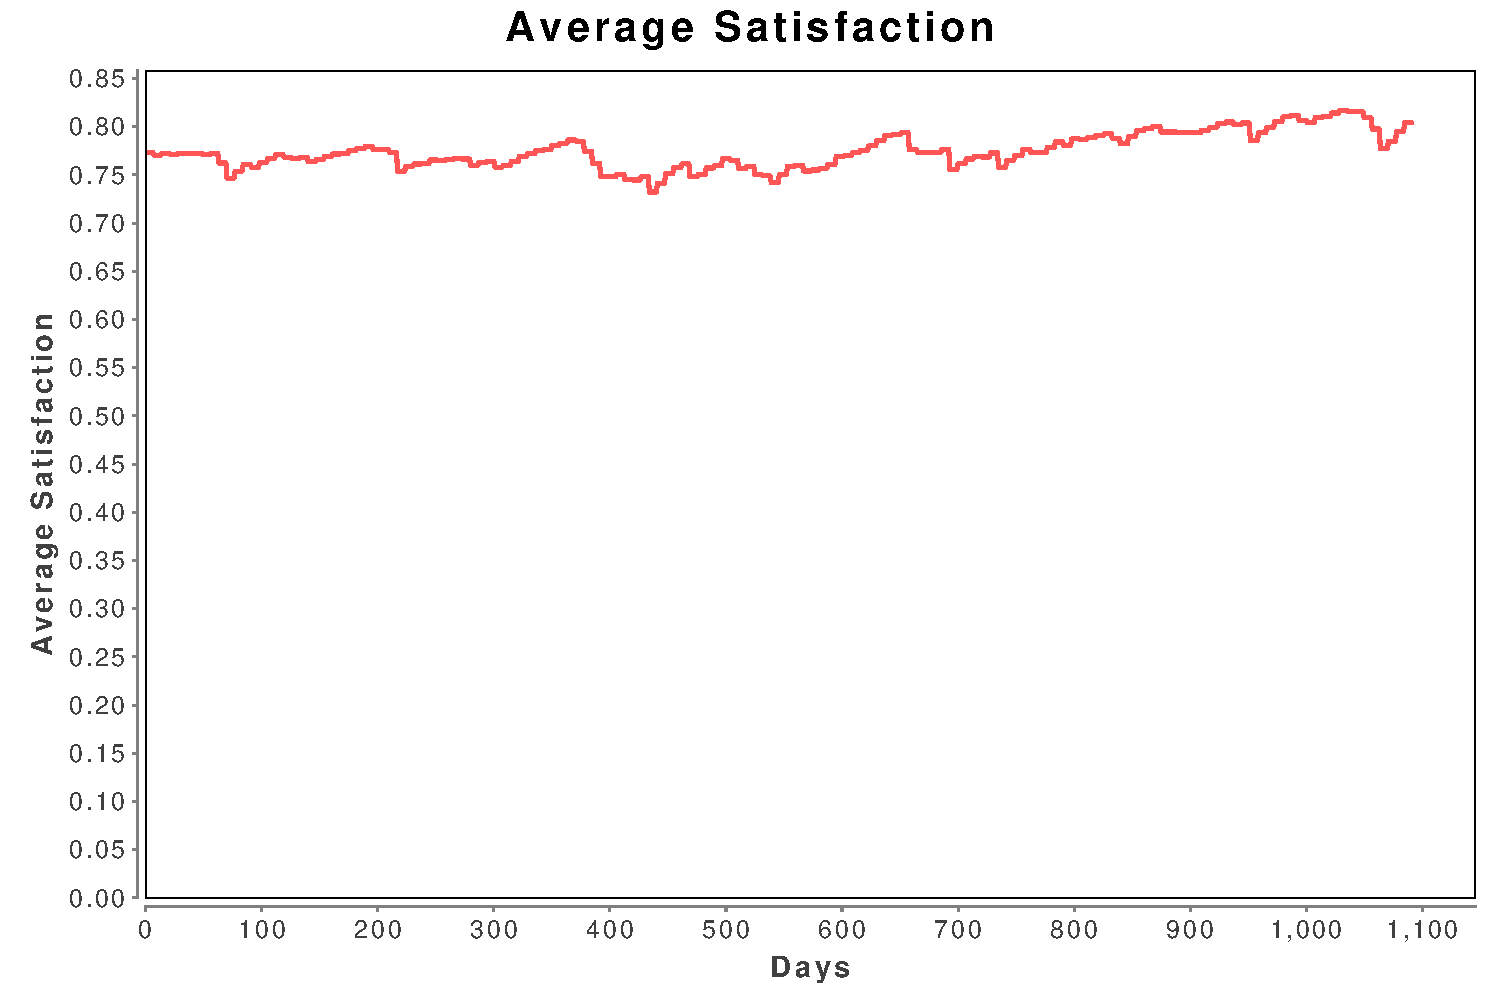
\includegraphics[width=2.25in,keepaspectratio]{average-satisfaction-new.pdf}\\
		After\\ Optimzation
	\end{columns}
\end{frame}
%%
\begin{frame}	
	\frametitle{Results: The Overall Situation}
	\begin{columns}[c]
	\column{2.5in}
		\centering
		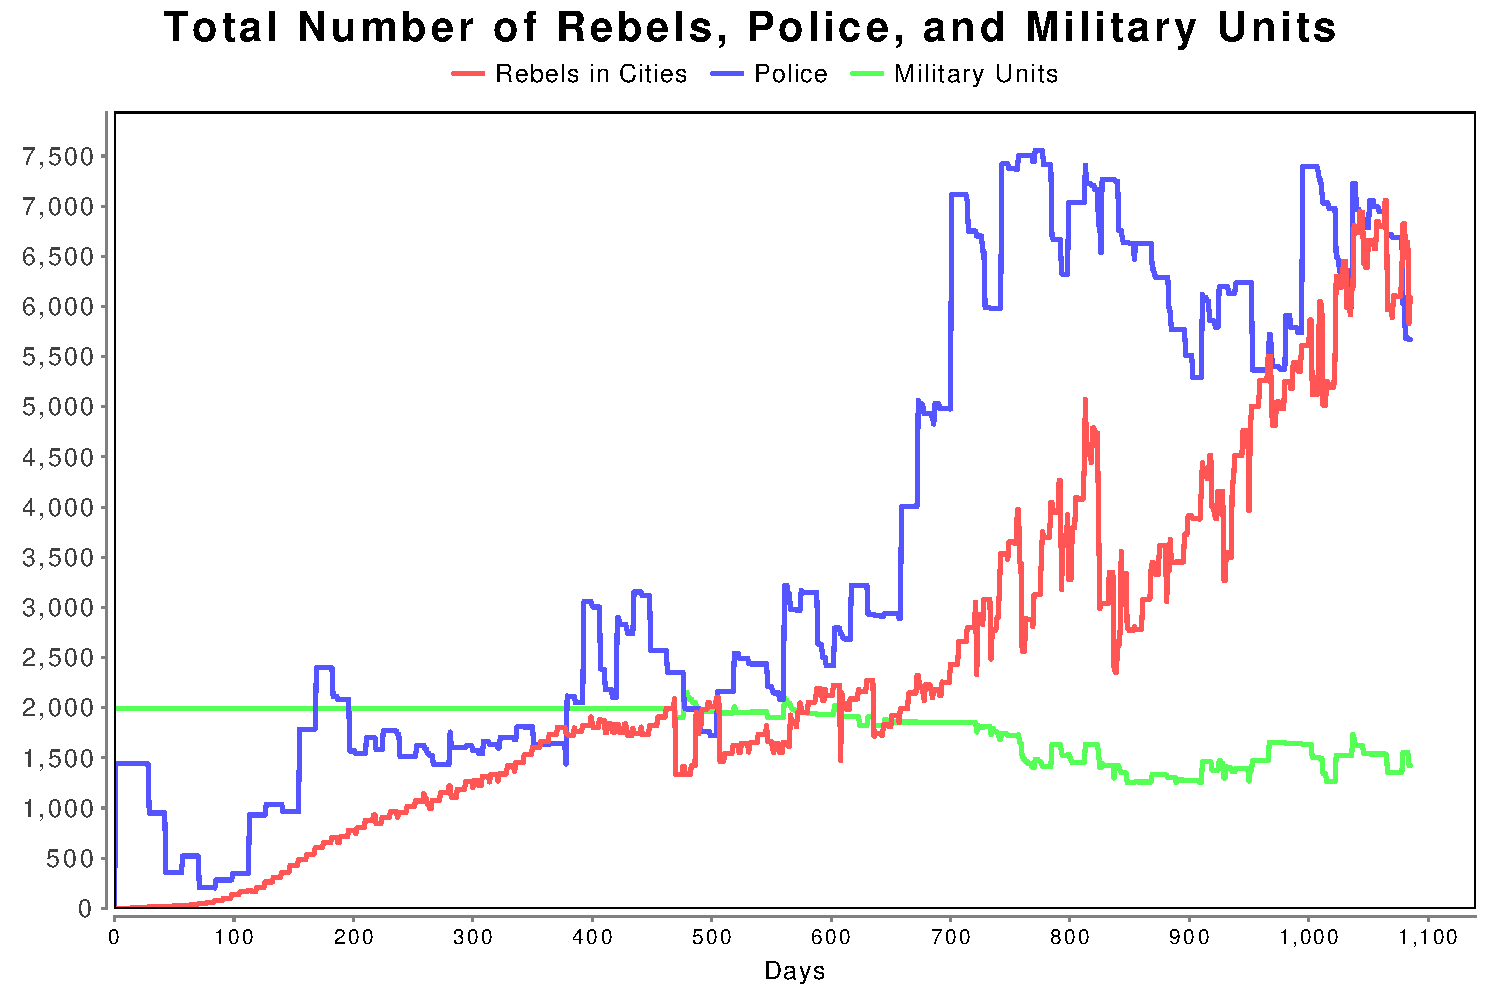
\includegraphics[width=2.25in,keepaspectratio]{situation-old.pdf}\\
		Before Optimzation \\(Original Parameters)
	\column{2.5in}
		\centering
		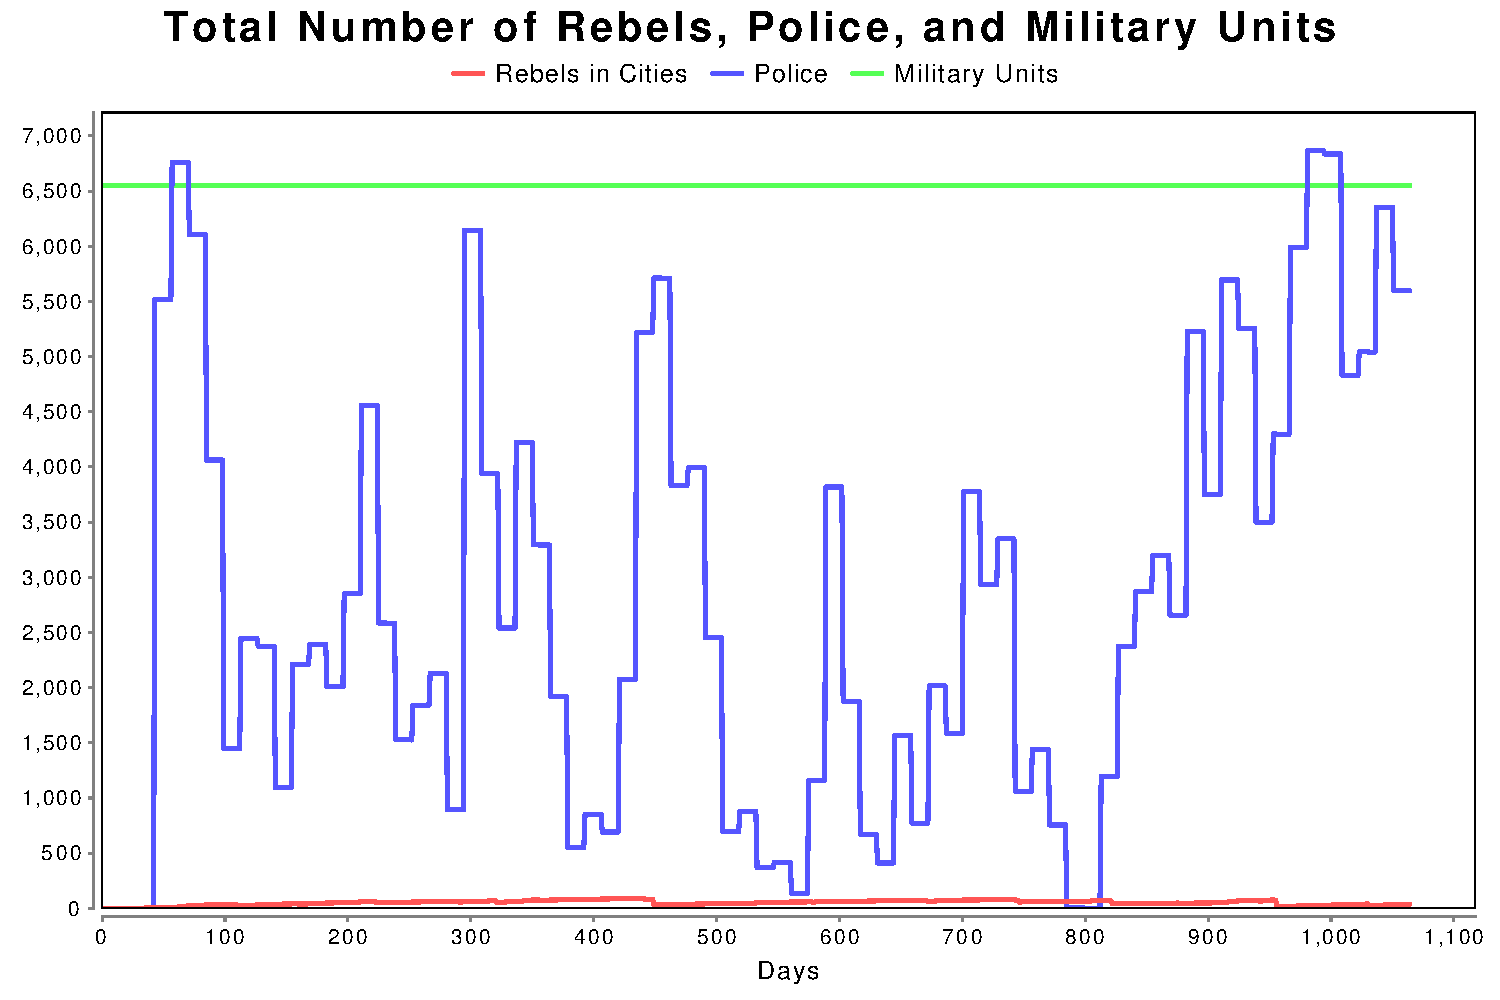
\includegraphics[width=2.25in,keepaspectratio]{situation-new.pdf}\\
		After\\ Optimzation
	\end{columns}
\end{frame}
%%
\begin{frame}
	\frametitle{Results: Some (interesting) numbers}
	\begin{itemize}
		\item State's corruption rate -- \textbf{86\%} 
		\item State's tax rate -- \textbf{77\%}
		\item State's maximum reserve rate -- 84\%
		\item State's minimum reserve rate -- 77\%
		\item Minimum benefit share to the populace (i.e. public spending) -- \textbf{98\%}
		\item Maximum number of police force per capita -- \textbf{31\%}
		\item Initial reserve army ratio -- 0.01\%
		\item Standing army size -- 0.06\%
		\item State's attack frequency (to suppress rebels) -- \textbf{78\%}
	\end{itemize}
\end{frame}
%%
\begin{frame}
	\frametitle{Conclusions}
	\begin{block}{Lesson ?}
		It's \textbf{fine} to run a \textbf{corrupt} government and keep its people \textbf{happy} -- \emph{only} if you have a \textbf{high} public spending, \textbf{large police force} and a very \textbf{frequent attack} on rebels.
	\end{block}
	\begin{block}{Utopia ?}
		These results are ``interesting'' -- i.e. \textit{communist dictatorship} ?
	\end{block}
	\begin{block}{Revelations ?}
		Does this reveal cracks in the \emph{RebeLand} model semantics? Or a bug in the code?
	\end{block}
\end{frame}
%------------------------------------------------
\section{Summary}
\begin{frame}
	\frametitle{Summary}
	\begin{columns}[c]
		\column{2.5in}
			\centering
			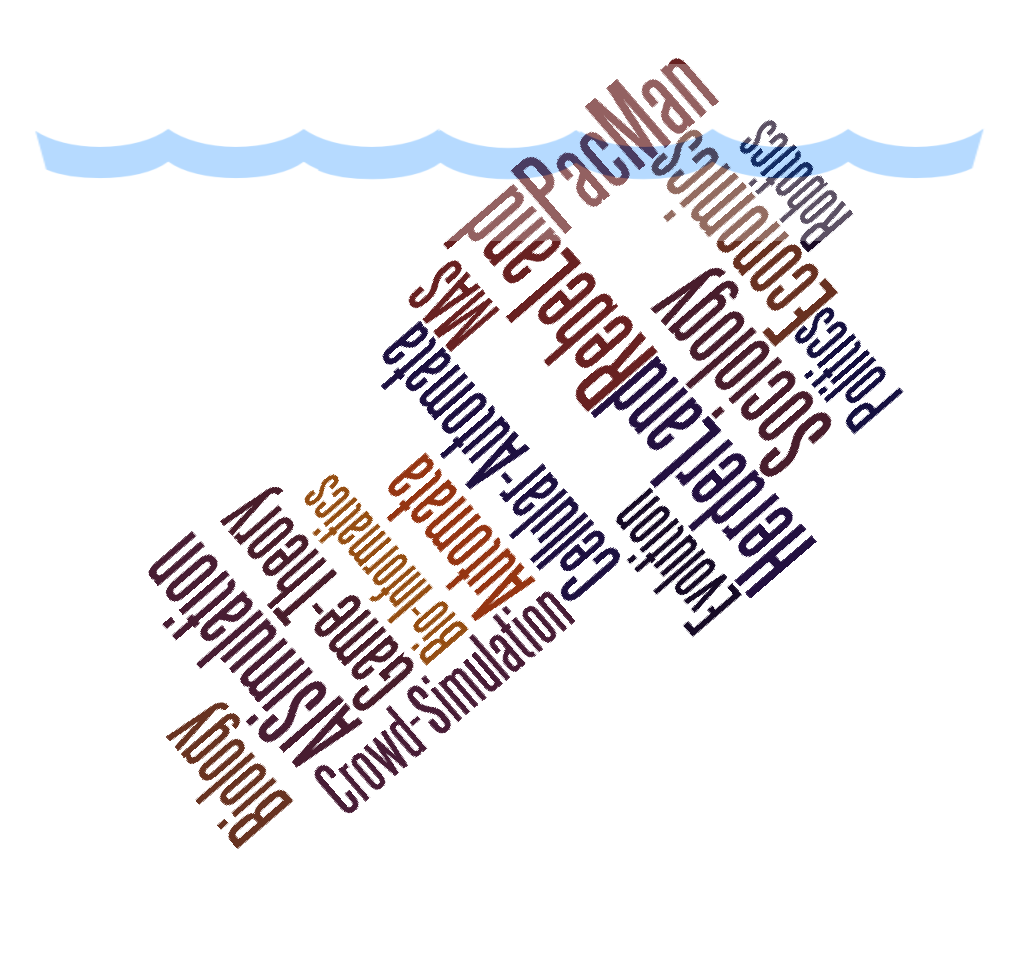
\includegraphics[width=2.5in,keepaspectratio]{iceberg.pdf}
		\column{2in}
		\begin{footnotesize}
			\begin{itemize}
				\setlength{\itemsep}{0.30cm}
				\item ECJ and MASON can be used to conduct many interesting experiments.
				\item Surely, symbiosis between MASON and ECJ -- has a lot more to offer.
				\item Building a unified/standardized APIs to help plugging ECJ capabilities into MASON models -- could just be a tip of the iceberg.
			\end{itemize}
		\end{footnotesize}
	\end{columns}
\end{frame} 
%------------------------------------------------
%------------------------------------------------
\section{Feedback}
	\begin{frame}
		\begin{block}{}
			\Huge{\centerline{Questions?}}
		\end{block}
		\begin{block}{}
			\Huge{\centerline{Discussions?}}
		\end{block}
	\end{frame}
%------------------------------------------------
\end{document} 
